\documentclass{article}

% DIMENSIONE PAGINA
\usepackage[a4paper,top=2cm,bottom=2cm,left=2cm,right=2cm,marginparwidth=1.75cm]{geometry}

%LAYOUT PAGINA
\usepackage{fancyhdr}
\pagestyle{fancy}
\fancyhead[R]{Fog and Cloud Computing}
\fancyfoot{}
\fancyfoot[C]{\thepage}
\fancyhead[L]{\leftmark}

\usepackage[utf8]{inputenc}
\usepackage{longtable}
\usepackage{graphicx}
\graphicspath{ {./images/} }
\usepackage{float} %Per posizionamento H


\usepackage{hyperref} %per TOC linkable

\hypersetup{
    colorlinks,
    citecolor=black,
    filecolor=black,
    linkcolor=black,
    urlcolor=black
}


% PER paragraph
\newcommand{\myparagraph}[1]{\paragraph{#1}\mbox{}\\}

% Ridefinizione spazio liste
\usepackage{enumitem}
\setlist{nolistsep}
\setlist{itemsep=0pt,parsep=0pt,topsep=4pt,partopsep=2pt}

\usepackage{placeins} %per float barriers


\begin{document}

\begin{titlepage} %crea l'enviroment
\begin{figure}[t] %inserisce le figure
    \centering
\includegraphics[scale=0.1]{images/unitn.png}
\end{figure}
\vspace{20mm}

\begin{Large}
 \begin{center}
	Dipartimento di Ingegneria e Scienza dell'Informazione
	
	\textbf{Corso di Laurea Triennale in Ingegneria Informatica, delle Comunicazioni ed Elettronica}
	
	\vspace{5mm}

    \hrulefill
    
    \vspace{25mm}
	
    {\LARGE{Appunti delle Lezioni}}\\
	\vspace{10mm}
	{\huge{\bf Fog and Cloud Computing}}\\
\end{center}
\end{Large}


\vspace{36mm}
%minipage divide la pagina in due sezioni settabili
\begin{minipage}[t]{0.47\textwidth}
	{\large{\bf Autori:\\Davide De Martini\\ Samuel Casagrande Cecchin}}
\end{minipage}
\hfill
\begin{minipage}[t]{0.47\textwidth}\raggedleft
	{\large{Professore: \\Domenico Siracusa}}
\end{minipage}

\vspace{25mm}

\hrulefill

\vspace{5mm}

\centering{\large{\bf Anno Accademico 2021/2022 }}

\end{titlepage}

\renewcommand*\contentsname{Chapters}

    \tableofcontents
    
    \section{Introduction}
\subsection{Introduction to cloud computing and fog computing}
Nowadays we live in a world of data, we create a lot of data per day and we have the need to access, share and process these data from all devices. This beacause analysing data reflects reality. There's a science that analyse data, it's called Data Science (Statistics, Machine Learning, Data Mining ecc.), with this science we are able to analyse data, create models and predict the future in a certain scenario. 

So now we know that we create a lot of data per day but how we use that data? We need a \textbf{distributed and scalable} system to do it. 

A solution for this is a \textbf{Data Center}, is a large distributed warehouse owned tipically by a large company (like Microsoft) full of "servers" that offer services to the customers. This business model work because companies are able to transform cost monetizing their hardware with services, they provide services to customer giving the possibility to have a good infrastructure without owning any server or stuff like this.

Not everyone can create a Datacenter
\begin{itemize}
    \item Is difficult
    \item Require knowledge 
    \item It cost 
\end{itemize}

The goal of \textbf{Cloud Computing} is to give the opportunity to everyone to have their own "infrastructure" 
So what is Cloud Computing? Cloud Computing is the trasformation of IT from product to service.

Cloud Computing has to be:
\begin{itemize}
    \item With shared resouces: the resources aren't dedicated (in most of the cases)
    \item Broad network access: available from anywhere with an internet connection
    \item On demand: consumer can reserve resources as needed (no human interaction with cloud service provider)
    \item Elatic: resources can be rapidly scaled up and down based on the demands
    \item Pay by use: User pay only for used services and can cancel any time the services
\end{itemize}
One of the first cloud solution was from salesforce.com (1999) which introducted applications delivered via a website, in 2002 Amazon Web Services (AWS) provides services like storage and computation. In the next years (2006) Elastic Compute cloud (EC2) was released: a commercial web service that allows small companies and individuals to rent compute capabilites over which they can run their own applications. Next google docs and office 365 were released.

So is cloud computing a new technology?
\begin{itemize}
    \item \textbf{No:} technology used are not new
    \item \textbf{Yes:} Is a new delivery model!
\end{itemize}
Let's see some differences between Traditional IT and Cloud Computing
\begin{center}
    \begin{longtable}{|c|c|}
    \hline
        Traditional & Cloud  \\
        \hline
        Manually provisioned & Self-provisioned \\ 
        Dedicated hardware & Shared hardware \\
        Fixed capacity & Elastic capacity \\
        Pay for capacity & Pay for use \\
        CAPEX\footnote{Money spent for phisical goods} and OPEX\footnote{Money spent for mantaining the service} & OPEX \\
        Managed via SysAdmin & Managed via APIs \\
        \hline
    \end{longtable}
\end{center}
The cloud ecosystem is made by:
\begin{itemize}
    \item Delivery models (SaaS, PaaS, IaaS ...)
    \item Deployment models (Public, Private, Community, Hybrid)
    \item Infrastructure (Distributed infrastructure, Resource virtualisation, Autonomus system)
    \item Resources (Compute e storage servers, Networks ...)
    \item Defining attributes (Elasticity, Pay-per-usage ...)
\end{itemize}
\begin{figure}[bh]
    \centering
    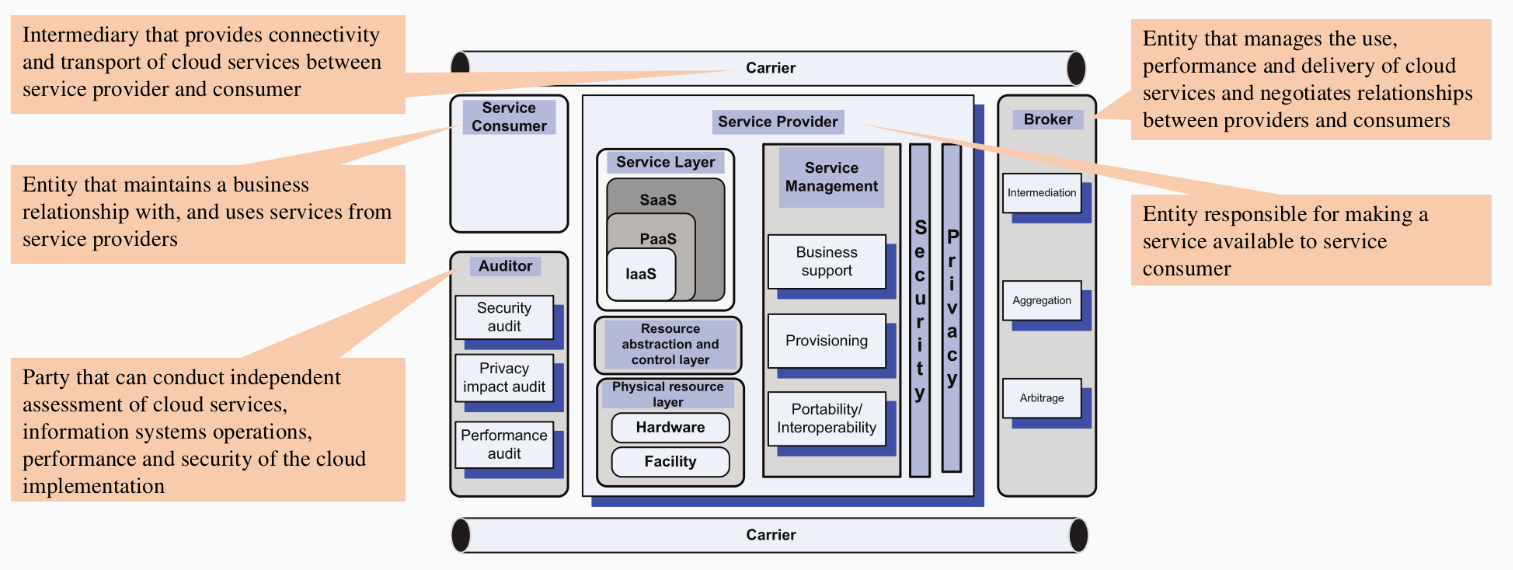
\includegraphics[scale=0.25]{images/cloudcomputingmodel.png}
    \caption{The NIST reference model for Cloud Computing}
    \label{fig:cloudmodel1}
\end{figure}
The NIST reference model for Cloud Computing is explained in figure \ref{fig:cloudmodel1}.

We spoke about \textbf{virtualisation} but what this term mean?
Virtualisation is the technique that abstract the computer resources, basically it isolate the hardware from the software and it make it possible to run different OS in the same infrastructure (like VirtualBox\footnote{An Oracle software for virtualisation and VM} for example). Let's see the difference between a Single and \textbf{Multi tenancy}:
In single tenancy each customer has its own software instance and requires a dedicated set of resources to fulfill the need of a customer. In a multy-tenancy environment instead of a single software instance a single instance of software runs on a server and serve multiple tenants, the resources management and costs are shared among tenants. With multi-tenancy you control a specific service without owning!

Another main feature of Cloud Computing is the \textbf{elasticity}, it means the ability to add or remove resources matching the workloads much more closely, it reduces the risk of overprovisioning and underprovisioning (we cancel idle time and the traffic overload). The risk of uderprovisioning is called \underline{transference of risk} we want to avoid that beacuse if users find that our service are unreachable there's the possibility of losing them (it happend in the past). In the other case, if we overprovision we pay for something that we don't use. The figure \ref{fig:elastic} is an example of the elasticity.
\begin{figure}
    \centering
    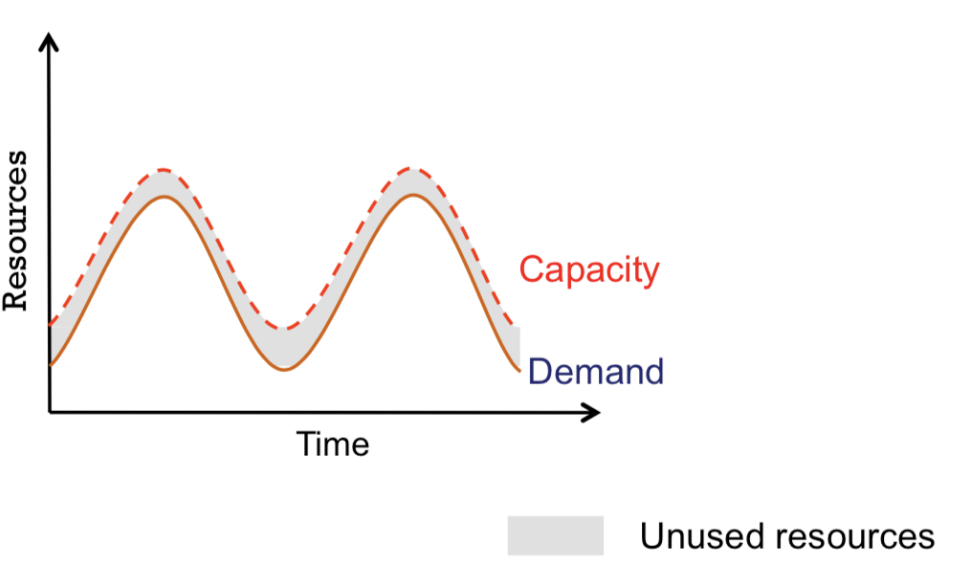
\includegraphics[scale=0.25]{images/elasticity.png}
    \caption{Example of elastic behaviour}
    \label{fig:elastic}
\end{figure}
\subsection{Cloud deployment models and delivery models}
The \textbf{deployment model} represent a specific type of cloud environment, distinguished by ownership, size and access
\begin{itemize}
    \item \textbf{Public} cloud: Are the providers like Google Microsoft or Amazon, their customers are the general public or a large industry group. They sell cloud services and manage the infrastructure. They are, of course, multi-tenancy
    \item \textbf{Private} cloud: It's for an exlusive use of an organisation, the infrastructure is located in the organisation or another party and it can decide if remotely host or not data
    \item \textbf{Community} cloud: It's for research community, is very similar to the Private cloud model
    \item \textbf{Hybrid} cloud: a mix of two or three model
\end{itemize}
The \textbf{Delivery models} define what "type" of service is offered, we have 3 big group
\begin{itemize}
    \item \textbf{Software-as-a-Service (SaaS):} These are the services like Netflix, Gmail. The user does not manage or control the infrastucture or the individual application (see figure \ref{fig:XaaS}), he only use the application to do things, this solution isn't good forreal-time applications.
    \item \textbf{Platform-as-a-Service (PaaS):} Allows a cloud user to deploy applications using programming languages and tools supported by the service provider. The user control the application but not the infrastructure under it (see figure \ref{fig:XaaS}).
    \item \textbf{Infrastructure-as-a-Service (IaaS):} With infrastructure we mean resources (like CPU, storage..), the user is able to deploy arbitrary software like OS and applications (see figure \ref{fig:XaaS}). IaaS exaples are server hosting, computing hardware, virtual instance (an example is EC2 from AWS)
    \item Others: like Hardware-as-a-Service, Database-as-a-Service (X-as-a-Service)
\end{itemize}
\begin{figure}[h]
    \centering
    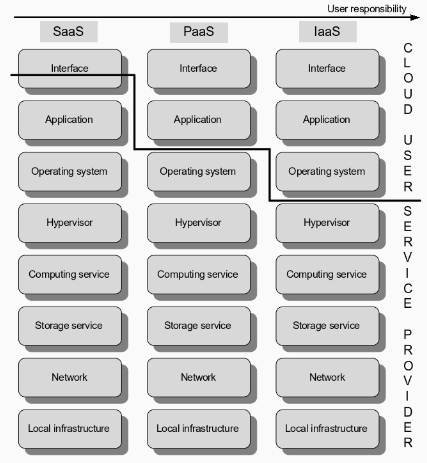
\includegraphics[scale=0.3]{images/XaaS.png}
    \caption{User control of the infrastructure}
    \label{fig:XaaS}
\end{figure}
\subsection{The market of cloud/fog solutions}
Speaking about real solution we can find three big OTT\footnote{Over The Top: the big company of computing}: Amazon which is a pioneer in IaaS (EC2 ecc.), Google which their efforts are focused in SaaS and Paas and Microsoft which its main involvement started with PaaS. Besides these big companies the market offers Open-source solution like OpenStack, OpenNebula ecc. In the first time the most of the revenue of cloud computing was generated by IaaS solutions and the market leader was AWS (and the same is nowadays). Amazon offers cloud services through a network of data centers on several continents, the regions do not share resurces and communicate through the Internet. When we buy an instance in practical we buy a virtual server with a well specified set of resources (CPU, storage ecc..). The user can choose the region where the virtual server should be placed and the instance type. When lauched the instance has a private IP address and a public one. In this process AWS get the request from the user, retrives a disk image of a VM and setup and locate the instance, last but not least give a IP address (through DHCP) and a MAC address. The user can interact using a Management Console, the SDK or using REST\footnote{Use HTTP request to communicate with the instance} requests.

    \section{Cloud technologies}
Initially virualisation was thinked to solve a big problem: consolidate multiple apps on a single server. This because the "one application per sever" it's a waste of money and resources.
\subsection{Virtualisation}
\textbf{Computing virtualization} is a flexible way to share hardware resources (CPU, memory, storage ..) between different operating systems.
\begin{figure}
    \centering
    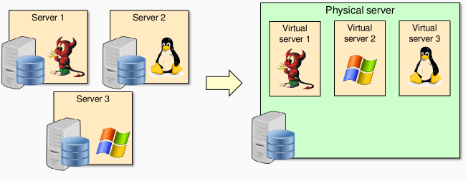
\includegraphics[scale=0.5]{images/virualisation.png}
    \caption{A virualization example}
    \label{fig:virt}
\end{figure}
So with virualization we use only one machine to run different OS and application (figure \ref{fig:virt}). The evolution of networking and the advent of optical fiber give the possibility to cloud computing to rise and became famous. 

Vitrualization has many pros:
\begin{itemize}
    \item \textbf{Isolation}
    \begin{itemize}
        \item Critical application could run in different and easily isolated OS
        \item Different services could run on the same hosts with an improved degree of isolation, we can assign a CPU core to one machine or isolate an application from the others to prevent issues caused by bugs or malicuious applications
    \end{itemize}
    \item \textbf{Consolidation}: Different OSes could transparently run on the same hardware at the same time saving hardware resources and money
    \item \textbf{Optimize energy consumption}: One machine running \textit{n} application use less electric energy than \textit{n} machines running one application
    \item \textbf{flexibility and agility}: Complete control over the execution information of all VMs, possibility to pause, resart, migrate and give more or less resources to the VMs
    \item \textbf{Possibility to duplicate a running VM}: For example to divide the traffic between two different machines
    \item \textbf{Disaster recovery}: Create snapshot and do rollbacks ecc.
    \item \textbf{Rapid deployment}: It's faster to deploy a VM instead of create a dedicated server for each service
\end{itemize}
Virtualization also brings with it limits and the challenge is try to handle it
\begin{itemize}
    \item \textbf{Additional overhead}: Each application has its own OS running (it use a lot of resources), however the overhead is usually considered acceptable for a wide range of different applications
    \item \textbf{More difficult to handle heterogeneous hardware}
\end{itemize}
There are tipically two scenarios of using the virtualisation technique, one is \textbf{Server virualisation} and the other is \textbf{Desktop Virtualisation} (like virtualbox), economicaly speaking server virtualisationis more important, desktop virtualisation is not a huge economic driver (most of this software is free). With virtualisation it's not important to have a physical machine with a given set of characteristics, we can create dynamically a virtual server with the requested characteristics. Users can buy tons of equivalent servers, with exactly the same hardware characteristics and aggregate them together in a datacenter and virtualize their resources.

Now let's see some definitions:
\begin{figure}
    \centering
    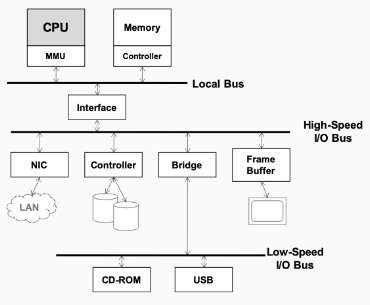
\includegraphics[scale=0.75]{images/computer architecture.png}
    \caption{Computer architecture}
    \label{fig:comparch}
\end{figure}
In figure \ref{fig:comparch} there explained the "normal" architecture schema of a computer, the goal of virtualisation is to \textbf{layer} all the things to create a modular like thing. Layering is a common approch to manage system complexity: it minimizes the interactions among the subsystems, simplifies the description of the subsystem. 

A layering model in computer system is the following:
\begin{itemize}
    \item Hardware
    \item Software
    \begin{itemize}
        \item Operating system
        \item Libraries
        \item Applications
    \end{itemize}
\end{itemize}
\begin{figure}
    \centering
    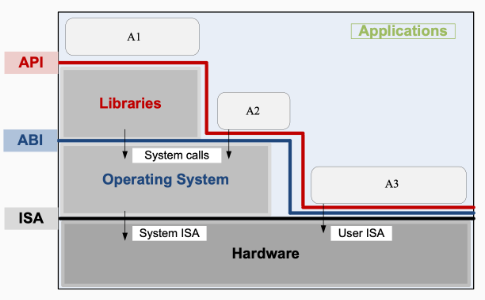
\includegraphics[scale=0.5]{images/layering.png}
    \caption{Layering schema}
    \label{fig:layers}
\end{figure}
As we see in figure \ref{fig:layers} an application use library functions (A1), makes system calls (A2), executes machine instructions (A3). This is possible because of three main interfaces (API, ABI, ISA)
\begin{itemize}
    \item \textbf{Instruction Set Architecture (ISA)}: Is at the boundary between hardware and software
    \item \textbf{Application Binary Interface (ABI)}: Allows application to access the hardware, it doesn't give privileged status but invokes system calls
    \item \textbf{Application Program Interface (API)}: Define the set of instructions the hardware was designed to execute and gives the application access to ISA
\end{itemize}
We spoke about \textbf{Virtual Machine} (VM) but what is it? A VM is a software emulation of a physical machine that executes OS and apps such as being in a physical one. The \textbf{Host OS} is the OS where the VM is running, is in charge of virtualise the hardware (it can include the Hypervisor). The \textbf{Guest OS} is the OS runned in the VM it doesn't know that is in a virtualised environment. The \textbf{Hypervisor} (or Virtual Machine Monitor) is the software in charge of the virtualisation process, it has to virtualise the resources. Virtualise means assigning a distinct set of resources to each VM and guaranteeing that each VM cannot get access outside its boundaries (in case resources cannot be partitioned arbitering the access to shared resources). So the Hypervisor manage virtualised hardware and system calls generated from Guest OS.

Computing virtualisation represent the most common approach for Cloud Computing according to IaaS model.


%-----------------------------------


\subsubsection{CPU Virtualisation}
We can ask the VMM to allocate many resources as many as we want and it will virtualize them.
The concept of virtualisation is different from the one of emulation:
\begin{itemize}
    \item[--] If the architecture of the virtual CPU is the same of the physical one, then the ISA (\textit{Instruction Set Architecture}) can be the same one (or a subset). We are in a case of \textbf{virtualisation}.
    \item[--] Otherwise if the virtual CPU's architecture is different from the physical one, then we talk about \textbf{emulation}. Emulation require the binary translation between the two ISAs and this is much slower.
\end{itemize}

We have alreay talked about VMs as \textbf{efficitent} (few overhead) and \textbf{isolated} (VMs don't step each other) copies of real machines.

We define the \textbf{Virtual Machine Monitor} (VMM) as a software that has to respect three charateristics:
\begin{itemize}
    \item It exports execution enviorments
    \item It executes some instrunctions on the real processor instead of on the virtual one.
    \item It should have complete control of the real system resources (but this not always happen)
\end{itemize}

There are three main different types of CPU virtualisation:
\begin{itemize}
    \item \textbf{Full virtualisation} where the guest OS can run unmodified. (ex VirtualBox).
    \item \textbf{Paravirtualisation} where the guest OS need to be modified in order to be executed
    \item \textbf{Hardware assisted Virtualisation} where the hypervisor exploit some hardware features (this method solved some issues from the other two solutions).
\end{itemize}

To isolate better the system we use a ring scheme. In x86 architectures there are often 4 rings that rapresent a privilage level. The kernel works in the ring 0 (most privileged level), instead applications in the ring 4 (less privileged).
Some modern OS uses just level 0 and 3 in order to reduce overhead and increase the CPU speed.
\begin{figure}[h]
    \centering
    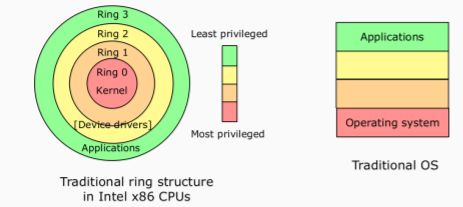
\includegraphics[scale=0.75]{images/rings.png}
    \caption{traditional ring structure of x86 Intel CPUs}
    \label{fig:ringstruct}
\end{figure}
When an application tries to run some instructions not available by the privilage level, the CPU handles them and execute a \textbf{TRAP command} that is a particolar INTERRUPT that move the execution to another ring (making a context switch).

Now the answer is where to put our guest OS.
There are two models:
\begin{itemize}
    \item The 0/1/3 (host, guest, application) model is problematic because the guest OS can run some instructions that it shouldn't and it can interfere with the VMM
    \item The 0/3/3 (host, guest, application) model solve the previous problem but is problematic because the guest OS is no longer protected from malicious applications that run over it.
\end{itemize}

There are two particular instructions that we have to menage in order to create a good isolation:
\begin{itemize}
    \item \textbf{Privileged instruction} are CPU instructions that generates TRAP routines if the CPU is running in the wrong context (For example using the system call HALT in ring 3, \textit{no privileges}).
    \item \textbf{Sensitive instructions} are CPU instructions that provide some information about the physical state of the processor (ex. its privileged level). If we want to virtualize a guest OS we want these instructions to be privileged.
\end{itemize}

We invoke \textbf{TRAP} routines when:
\begin{itemize}
    \item We try to execute instructions not allowed (Exceptions)
    \item System calls are invoked
    \item There are hardware INTERRUPTs.
\end{itemize}
In the OS there are memorized groups of instructions to be executed for every type of INTERUPTs (\textbf{Interrupt Description Tables}, IDT). In traditional way, when a TRAP routin is invoked, the CPU jumps to these tables (with a \textbf{IRET\footnote{This technique is very slow, it parse several memory location} instruction}) and execute indicated instructions in a privileged way. This is a context switch and it has a cost! The new way uses is more performing, it uses specific registers to store the routine and then calls SYSENTER and kernel runs in a very fast transition.

In an emulated environment the guest OS runs in an unprivileged environment (as an application). If it requires an instruction not allowed, the CPU launches a TRAP that the VMM intercepts. After that the VMM emulates the instruction and gives control back on the guest OS execution that will try to handle it. 
Thanks to this method the guest OS can execute some operations (like shutting down) because of the VMM emulation. So the guest OS keeps not knowing that is running over a VM.
\begin{figure}[H]
    \centering
    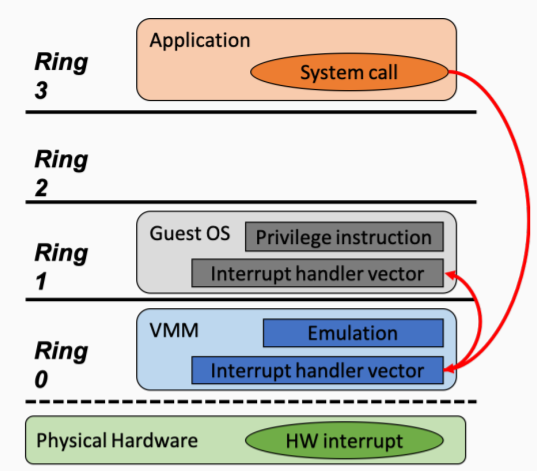
\includegraphics[scale=0.37]{images/trap in emulation.png}
    \caption{trap routine in emulated OS}
    %\label{fig:ringstruct}
\end{figure}
If the handle instruction needs to execute others privileged instructions (applications use library that provides functions) it will give control back to the VMM (invoking a new trap)
\begin{figure}[H]
    \centering
    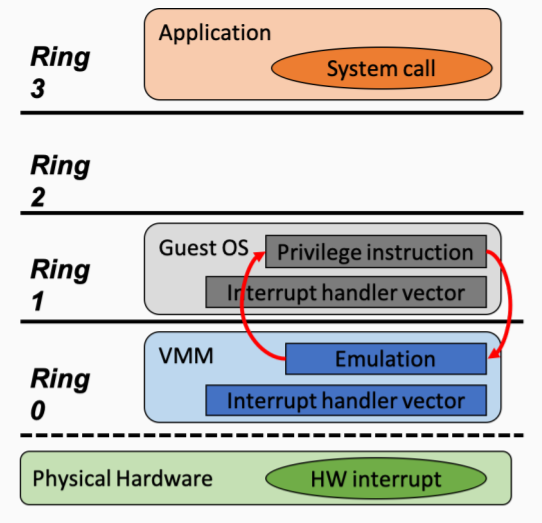
\includegraphics[scale=0.37]{images/trap in emulation (2).png}
    \caption{trap routine in emulated OS (2)}
    %\label{fig:ringstruct}
\end{figure}
If the TRAP is caused by an hardware INTERRUPT, CPU invoke the VMM interrupt handler; the VMM then will jump to the interrupt handler of guest OS.
\begin{figure}[H]
    \centering
    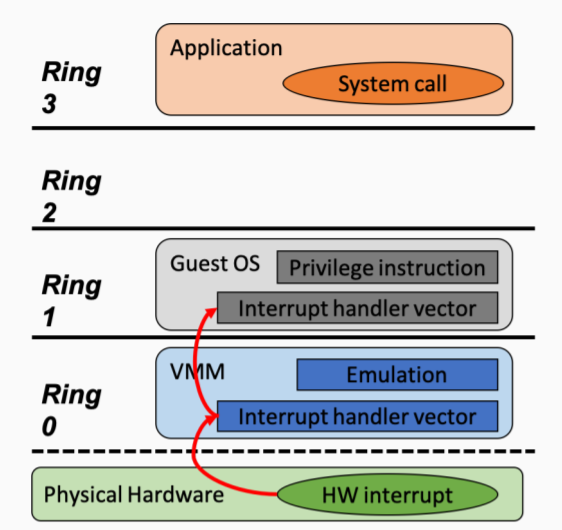
\includegraphics[scale=0.37]{images/trap in emulation (3).png}
    \caption{trap routine in emulated OS (3)}
    %\label{fig:ringstruct}
\end{figure}
The \textbf{trap and emulation} paradigm that we have just discussed has two problems:
\begin{itemize}
    \item It causes huge costs in terms of time-consuming; in fact the CPU has to switch between privilege levels many times for every TRAP invoked.
    \item Many architectures are not made to be virtualized. They have some sensitive instructions that don't trap if executed (so the VMM can't detect them).
\end{itemize}
Let's see some possible solutions:
\begin{itemize}
    \item Detect and interpret them dynamically (very long and slow process)
    \item Use \textbf{Dynamic Binary Translation} (DBT): this doesn't require any OS modifications or hardware supports. The VMM dynamically (at runtime) translate sensitivity instructions in instructions that trap. This causes hight overhead that can be reduced introducing caching techniques. \textbf{Vmware wokrstation} is a combination of Trap and Emulation paradigma and the DBT; it makes possible to push the guest OS to the ring 1 and the VMM to ring 0.
    \item Change the OS patching it (this is a long elaboration). This is called \textbf{Para-Virtualisation}: the guest OS is explicitly deprivileged (to ring 1) but is enriched with some mechanism to communicate with the hypervisor (particular hypervisor calls). This is a faster solution (it doesn't need to emulate stuff) but require OS modifications. It's not compatible with Windows OS.
    %\item Make all sensitive instructions privileged. 
    \item \textbf{Hardware-assisted virtualisation} (HVM). The idea is to have a hardware support that promote sensitive instructions as privileged or dynamically configure a trap mechanism (in the VMM). In particular CPU creates a new model of privilege levels (non-root mode) over the native one (root mode) and puts the guest OS on the lower level of non-root mode and on the ring 3 of root mode.
    \begin{figure}[H]
        \centering
        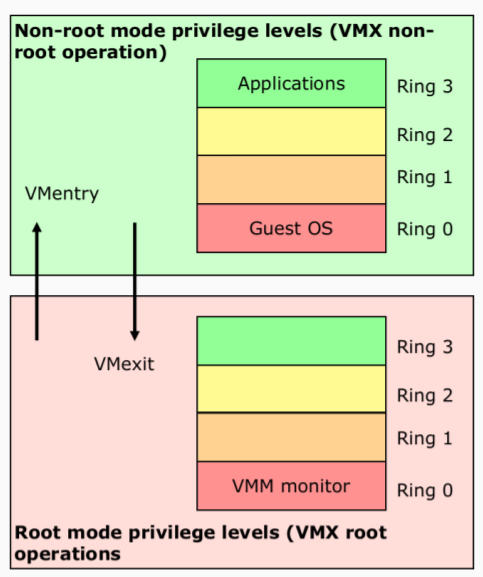
\includegraphics[scale=0.37]{images/HVM.png}
        \caption{HVM structure}
        %\label{fig:ringstruct}
    \end{figure}
    Through VMLAUNCH and VMRESUM instructions (VM exits) the CPU enters and exits from non-root and root mode in order to temporarily give the control to the VMM just to execute the privileged instruction (emulating the correct behavior). This solution introduce a great simplification: the time of trapping is reduced and the DBT method is avoided; Furthermore there's no OS modification.
    \begin{figure}[H]
        \centering
        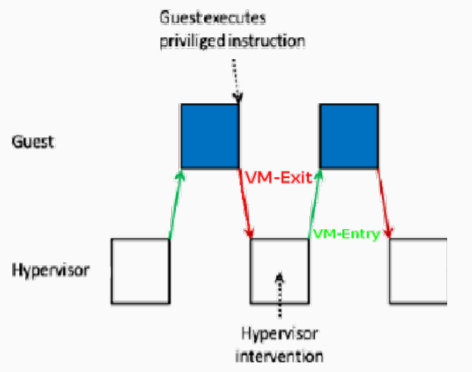
\includegraphics[scale=0.37]{images/VM exits.png}
        \caption{execution of privileged instructions in HVM}
        %\label{fig:ringstruct}
    \end{figure}
    The \textbf{Virtual Machine Control Structure} (VMCS) is a new element of memory that allows the switching between the two modes memorizing:
    \begin{itemize}
        \item Guest state (stored during VM exits and loaded during VM entry)
        \item Host Processor information
        \item Some control data
    \end{itemize}
    But there's still a problem: nested virtualisation is much slower because nested VMs can't use HVM.
\end{itemize}


\subsubsection{Memory virtualisation}
Modern Operating system use "memory paging" (the physical memory is interpreted into pages) to access as contiguous dispersed locations in the physical memory; the OS keeps a set of tables to translate the virtual memory address into physical ones (this operation is handled by \textbf{MMU}). Virtual addresses, used by processes (starting from 0), are translated by the MMU to physical addresses using big hash table for the mapping.

\begin{figure}[h!]
    \centering
    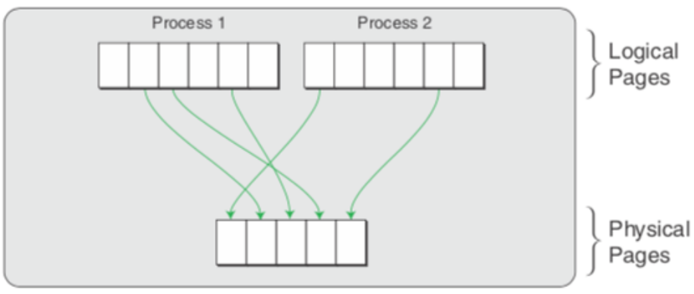
\includegraphics[scale=0.3]{images/mapping_mm.png}
    \caption{Mapping from LPNs to PPNs}
    \label{fig:mapping_mm}
\end{figure}

If we take a look at fig \ref{fig:mapping_mm} we see the walks that hardware does in order to determinate the corresponding physical address.

Another task of the MMU is to manage the \textbf{TLB} (\textit{Translation Lookaside Buffer}). This is a cache with very fast access that keep stored the association of recently used logical pages with  physical pages. When a process asks for a logical address the OS tries to find the association in this cache; if the result is missing than it will ask the MMU for it.

But why we would like to virtualize memory?
\begin{itemize}
    \item \textbf{Simplicity}: Every process gets illusion of whole address space (apps doesn't have to care about pages).
    \item \textbf{Isolation}: Every process is protected from every other.
    \item \textbf{Optimization}: The OS can optimize how pages are used; this reduces space requirements.
\end{itemize}

In VMs is required another level of translation (Guest virtual address $\rightarrow$ Guest physical address $\rightarrow$ Machine physical address). To avoid this step a "\textbf{Shadow Page Table}" is introduced: it stores and keeps track of the mapping between Guest logical address and Machine physical pages, it's invisible from the guest point of view and it'll be used by the CPU for a translation when the guest is active.

How it works:
\begin{itemize}
    \item The VMM maintains the association of physical pages and machine pages in internal data structures.
    \item The VMM stores associations of logical pages and machine pages inside shadow page table exposed to hardware.
    \item The TLB keeps stored most recently used logical pages and the correspondents machine pages.
\end{itemize}
\begin{figure}[h!]
    \centering
    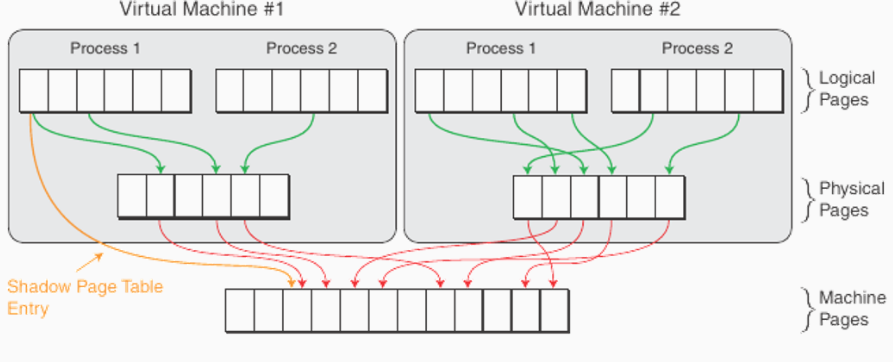
\includegraphics[scale=0.3]{images/mapping2_mm.png}
    \caption{CPU see only orange arrows, VMM see only red ones}
    \label{fig:mapping2_mm}
\end{figure}

The VMM is in charge of keeping the Shadow Page Table synchronized with the guest OS page table.
An important problem is the extra overhead that is introduced for keeping updated the Page Table when guest OS makes some updates in its ones. In order to avoid this overhead Intel and AMD have introduced two technologies (Extended Page Table and Rapid Virtualisation Indexing) that allow to do again a double translation: in fact traditional page tables translate logical pages into physical ones and the VMM maintains physical pages and machine pages mappings in an additional level of page tables, called \textbf{nested}.
\begin{itemize}
    \item Both the traditional page tables and the nested page tables are exposed to the CPU (now CPU know all the "path").
    \item Now there's no need to expose Shadow Page Tables, CPU does all the work (fig. \ref{fig:mapping3_mm})
\end{itemize}
\begin{figure}[h!]
    \centering
    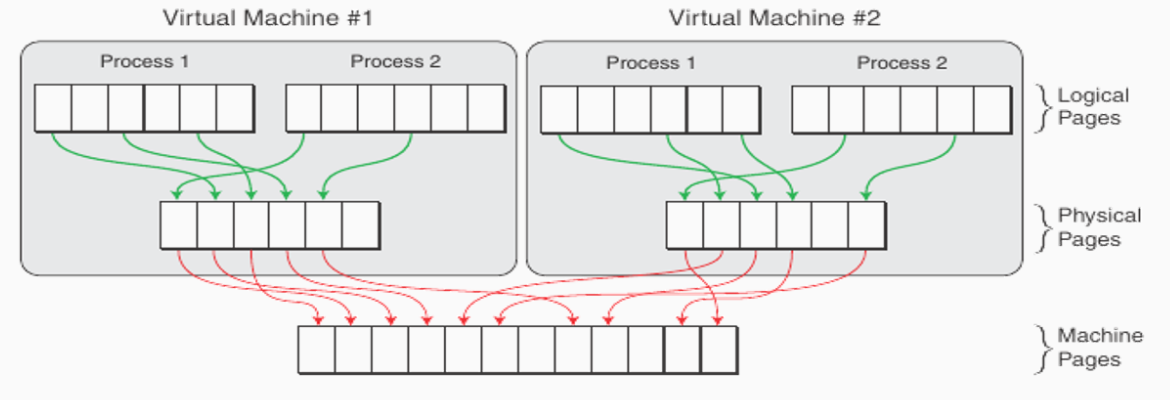
\includegraphics[scale=0.3]{images/mapping3_mm.png}
    \caption{Extended Page Table}
    \label{fig:mapping3_mm}
\end{figure}

This approach removes the need of VMExits (that involve context switches) associated with page table virtualisation. Guest could now keep update its page table without any overhead.

In addition to this now there's no need to use Shadow Page Table anymore; anyway this increases the cost of a single page walk; so now the TLB cache becomes critical to guarantee good performance (for example Intel processors uses two TLBs, one for normal pages and one for huge pages).

One last step to optimize memory virtualization technologies is to add an identifier for each virtual processor in order to allow several virtual processors coexist on the TLB at the same time (and don't leave the possibility to a processor to access to other processor caches).


\subsubsection{I/O virtualization}
As other resources, there are several techniques adopted for virtualizing I/O devices:
\begin{itemize}
    \item Device emulation
    \item Para-virtualized device
    \item Direct assignment
\end{itemize}
The choice of the technique depends on the type of device and if it Shared/Dedicated to a single Guest OS.

The problem with I/O devices is that every hardware manufacture does its devices as it wants. In order to make them working with every OS, they must provide \textbf{drivers\footnote{they standardise the method for the communication}}.

\myparagraph{Device emulation}
In \textbf{Device emulation} VMM proposes to the Guest OS an emulated device. The guest OS has no idea that is an emulated device (it just tries to do instructions that trap on the native OS) and the VMM has to remap device communication with the physical device in native OS (VMM has to emulate the response of the I/O for the Guest OS that doesn't care to the real drivers).
So the guest OS keeps using its drivers that are completely detached form the ones of native OS.

This approach is simple and easy to set up (and transparent to the guest OS): there's no need to install dedicated drivers and a single physical device could be multiplexed with several emulated device.
The disadvantage is that I/O operations are generally slower than physical ones and that could increase substantially the CPU load.

\myparagraph{Para-virtualization}
In \textbf{Para-virtualized device} guest OS is enriched with dedicated drivers (Guest OS knows that it's virtualized). It's very similar to CPU virtualization but in this case is simpler: it requires only to create new dedicated device drivers instead of modifying a kernel (making things easier and faster without having to fake anymore driver answers). In addition you need just a single para-virtualized driver for every device.
An example of usage of this method is realized by the Memory Ballooning driver. This is a special driver that stands besides traditional drivers and allow to communicate (directly to the VMM) how much memory is used in VM. This allows to make the memory allocation dynamic without over-committing.

\myparagraph{Direct assignment}
In \textbf{direct assignment} the VM communicate directly with physical I/O devices. In this case, the drivers used are the ones of the guest OS and not of the host OS.

\textbf{PCI-passtrough} is an example of application of this method. In particular it allows to use physical PCI devices (graphics card and network card) inside VMs.

Apparently the problem is always the same: how a device can write/read in the physical memory?
As we discussed above, the VMM perform some kind of translation (with relative overhead) from logical addresses to physical ones. \textbf{IOMMU} is an extension of the MMU that remaps addresses accessed by the hardware to the same table used to map guest-physical address to host-physical addresses.

Furthermore the PCI-e standard defines SR-IOV, a technology that allows to create a partition of the network interface card so that different parts can be assigned to different VMs.

In conclusion, direct assignment is the fastest and less expensive technique of I/O virtualization.


\subsection{Hypervisor architectures}
Traditionally there are two main kinds of architectures; a hybrid approach is sometimes used too.

\subsubsection{Type 1}
The hypervisor of type 1 runs directly on bare metal (hardware). On the top of it there are all guest VMs.
This is the type that guarantee best performances (because there is no OS in the middle) but that's quite complex in installation: in fact a hypervisor has less functionality of a real OS but needs to have the proper drivers for all hardware.
Most famous implementations are Vmware ESXi, Xen and Microsoft Hyper-V.

\subsubsection{Type 2}
The hypervisor of type 2 runs over a host OS as a common application. This is a less performing technique but easy to install and configure. Most famous implementations are VirtualBox and VMware workstation.

\subsubsection{hybrid type}
The hybrid hypervisor is implemented in the OS kernel (the host OS is the hypervisor itself). This technique allow very good performances.

\begin{figure}[h!]
    \centering
    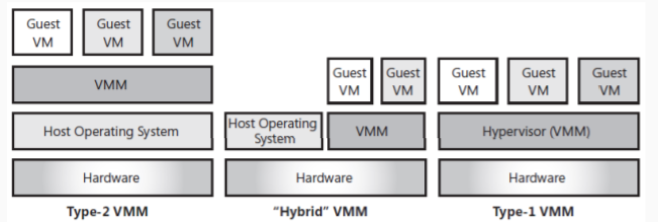
\includegraphics[scale=0.4]{images/VMM architectures.png}
    \caption{Graphical representation of VMM types}
    %\label{fig:mapping2_mm}
\end{figure}


\subsection{OS-level virtualisation}
Let's summarise VMs advantages:
\begin{itemize}
    \item they allow to run different OS on the same architecture
    \item they provide an isolated environment for single applications 
    \item excellent isolation with CPU and memory
\end{itemize}
and disadvantages:
\begin{itemize}
    \item Important overhead executing the guest OS (huge usage of CPU and memory)
    \item Necessity to constantly take care and keep updating hundreds of different OS
    \item more OS booting time
\end{itemize}

But do datacenters need to install multiple copies of same OS? It's more useful instead having a main OS (that's Linux) that share its kernel to different processes.
This is called \textbf{lightweight virtualisation}. In order to substitute VMs, it guarantees with less overhead:
\begin{itemize}
    \item scalability
    \item elasticity
    \item isolation
\end{itemize}

The idea is to run the OS virtualized without having a hypervisor (it's the Linux itself), replacing VMs with containers (virtual environments). Of course there are some limits compared to VMs but it's enough for lots of operations.

There are some requirements to implement lightweight virtualisation:
\begin{itemize}
    \item possibility to control resources (CPU cores, RAM) of physical machines among processes. In particular resources are dedicated to sets of processes.
    Working with groups of processes is better:
    \begin{itemize}
        \item you can menage and control them as a single class
        \item they are able to talk each other easily (for example inside the same application)
    \end{itemize}
    \item security and isolation (processes don't have to affect others). Isolation is so important for some reasons:
    \begin{itemize}
        \item a process must be always safely executed (with no possibility to compromise the entire machine), with some amounts of resources dedicated to.
        \item hardware isolation must be avoided; it will overkill all the technology.
    \end{itemize}
    \item possibility to menage an entire datacenter as a unique entity. This allows more portability
\end{itemize}

\subsubsection{Cgroups}
Linux kernel provides some primitives to limit, account (useful for billing), isolate and deny resources to processes or groups of processes.

Let's see main instructions:
\begin{itemize}
    \item \textit{cgcreate} create a cgroup
    \item \textit{cgset} set CPU.shares values to cgroups. They are relative values that make sense only with other values
    \item \textit{cgexec} execute the cgroup
\end{itemize}

Given two cgroups with 1024 and 512 CPU.shares, if the architecture has a single core, resources will be allocated with a proportion of 66\% and 33\%.
Instead if the architecture has multiple cores, resources will be allocated with a proportion of 100\% and 50\%.

\subsubsection{Namespaces}
\textbf{Namespaces} are virtual environments (highly related with cgroups) where processes visibility is limited to the partition itself (so two namespaces will have completely different IP addresses routine tabs, stacks, ...).

Currently there are seven different types of namespaces: IPC, Network, Mount, PID, User, UTS, Cgroup. Every type than can have multiple instances.
%DOMENICO UNO DI NOI\footnote{DOMENICO SIRACUSA CAPO DELLA TRAP PER FAVORE INGRAVIDACI} 

In Linux all processes are generated by a \textit{fork()} function invoking starting from the \textit{init()\footnote{nowadays called \textit{systemd}}} process. So processes generate other processes, creating a tree. A process with enough privileges and under some conditions can inspect another process by attaching a tracer to it or may kill/suspend it.

PID namespace enable multiple nested process tree (fig. \ref{fig:nestedtree}).
The main advantage of nested tree is that the first process of sub-tress will be seen as the "init" (PID 1) from its children (thanks to isolation).
The parent PID namespace know about all the processes; instead children ones don't know about the processes in the yellow area.
So a single process can now have multiple PIDs associated to depending from which which process/namesapce you are looking from. In particular the PID will be implemented as an array of values witch id/namespace association. This is an advantage also from the point of view of protection.

\begin{figure}[h!]
    \centering
    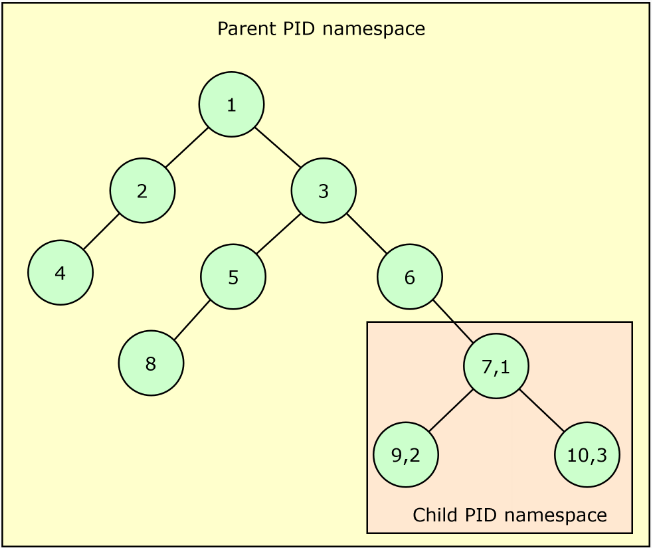
\includegraphics[scale=0.3]{images/processtree.png}
    \caption{An example of nested process with isolation}
    \label{fig:nestedtree}
\end{figure}

\myparagraph{Network Namespaces}
We saw that there are different namespaces for different kind of uses. Let's talk about \textbf{network namespace}. A \textbf{network namespace} allows two processes to perceive a completely different network setup (like routing table, interfaces, firewall, loopback ecc.). Once a network namespace is created we should create additional virtual network interfaces ($veth$) that allows traffic to cross namespace borders and to be delivered to another namespace (fig. \ref{fig:netnamespace}).

An example:
\begin{verbatim}
    sudo ip netns add <netsname> #create a new network namespace named <netsname>
    sudo ip link add veth0-root type veth peer name veth0-ns # Create virtual eth links
    sudo ip link set veth0-ns netns <netsname> #link the namespace to veth0-ns
\end{verbatim}
To interact in the namespace use the command:
\begin{verbatim}
    [sudo] ip netns exec <namespace_name> <command>
\end{verbatim}
After creating namespaces and the virtual "wire" between them and the server in which they are running, we have to assign IP-addresses:
\begin{verbatim}
    sudo ip addr 20.1.1.1/24 dev eth0
    sudo ip netns exec ns1 ip addr add ...
\end{verbatim}
Of course a root namespace is not enough to allow communication with the outside. In fact the server in most cases has a single public IP and multiples private IP. In order to translate private to public IP and forward communication the server needs the NAT.

Other examples of namespaces are:
\begin{itemize}
    \item \textbf{Mount namespaces} that enable the creation of a completely new file system (as a new volume)
    \item \textbf{User namespaces} that allow a process to have root privileges
    \item \textbf{IPC namespaces} that create private inter-process communications
\end{itemize} 

\begin{figure}[H]
    \centering
    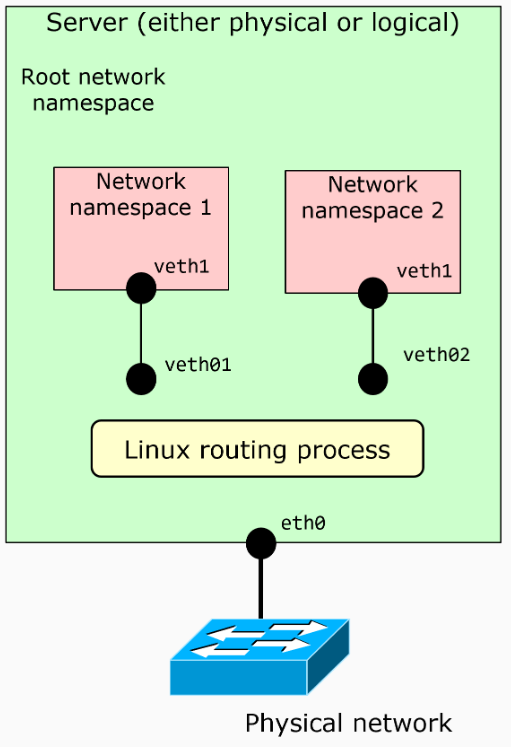
\includegraphics[scale=0.3]{images/netnamespace.png}
    \caption{Schema of a basic network namespace}
    \label{fig:netnamespace}
\end{figure}

\subsubsection{Limitation of these approaches}
Cgroups and Namespaces have some limitations:
\begin{itemize}
    \item beyond process isolation, they can provide a solution for a single server but it takes a lot of command to handle an entire datacenter (composed by hundreds of servers)
    \item they cannot guarantee application portability (such as in the case of VMs). On other computers you'll need to recreate all namespaces from zero
    \item Some commands are not so easy to use
\end{itemize}

\subsubsection{Linux containers}
A solution for cgroups and namespaces problems is \textbf{Linux containers} (LCX). They can provide a lightweight virtualisation (isolation without the complexity of full virtualisation). 
In particular they are an OS-level virtualisation method for running multiple isolated Linux systems on a single control host (the linux kernel is shared across all containers).

The main usage is to run isolate software. LSC allows to configure each container with the list of features it needs by means of a configuration file

Let's see the differences between Containers and Hypervisors in terms of consumes:
\begin{itemize}
    \item containers share the kernel with each other (it can be shared because it's rare that one app need a specific kernel). However the kernel is pretty small compared to libs and bins. So storage requirement is practically the same
    \item containers use less CPU
    \item containers use less memory (RAM)
\end{itemize}

Containers share the same operating system (kernel) as the host. Inside the box they look like a VM (or better a machine), but outside they look like normal processes. They don't emulate hardware and don't run different kernels. Security is not an out-of-the-box feature. Containers are faster and lighter than real VM (they can achieve the same performances of native execution with no virtualisation overhead) but in the other hand VMs provide better isolation, better security and give the possibility to use different OSs.

An overkill feature of the containers is that they are versatile.
\begin{figure}[h!]
    \centering
    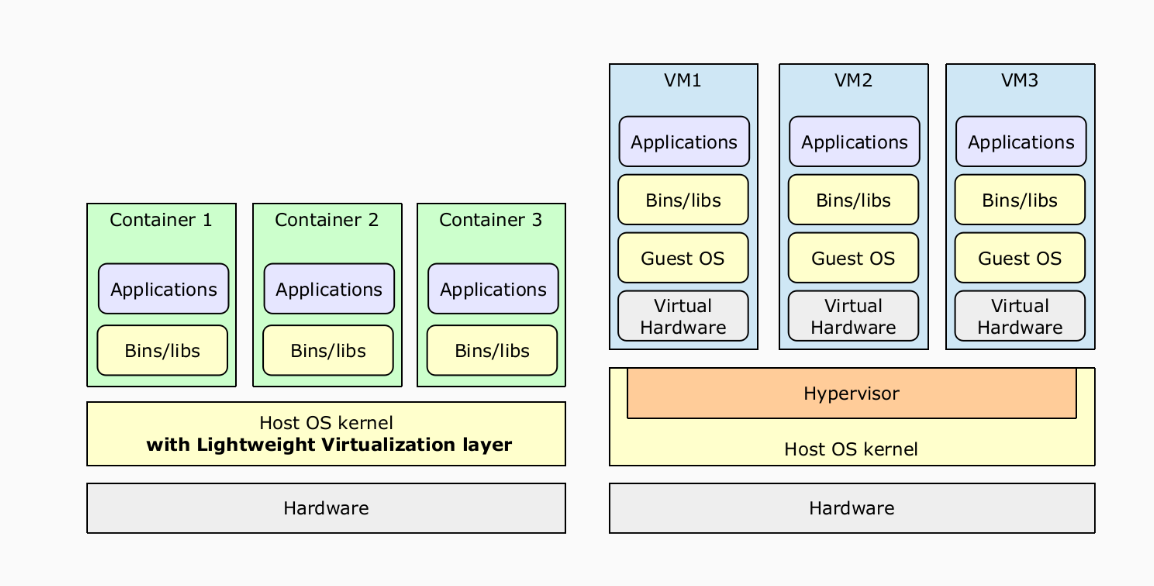
\includegraphics[scale=0.25]{images/contvshyp.png}
    \caption{Containers vs Hypervisors}
    \label{fig:cvs}
\end{figure}

However LXC have some limitations:
\begin{itemize}
    \item A container doesn't memorize the state of a machine. To make possible to migrate containers you should be able to copy and paste the machine state (there are some software tool but not 100\% working). Instead VMs have everything inside, the state too.
    \item There are some resources that you can't isolate completely (like transmission capacity; you can just do some policy)
    \item LCX can't be ported. You always need to create again the container from scratch. This is the most restrictive limitation because it prevent to move servers or stuff running in a container
\end{itemize}

\subsubsection{Docker}
\textbf{Docker} tries to solve the portability problem. It's a service that doesn't focus on virtualisation but directly on applications. Developers up to now had to package applications for each OS (with the possibility to make mistakes or to have other kind of problems); with Docker they can use a light environment (and portable too) that works everywhere they want (locally or in a server).

Docker provides a clean separation between environments and a set of instruction to menage them (it has a simple command line interface to menage containers). Docker containers can run with some TCP ports in order to communicate (Docker itself will create a networking environment that can be shared). However Docker is not a virtualisation engine and doesn't use hardware primitives.

Developers can creates containers and use libraries and dependencies in order to develop their applications. Sometimes they could want to hid code and data from the container (for example if the code is not open-source).

DevOps (who runs the container and uses applications) can login, access, configure and monitor applications that they use.

\myparagraph{Docker Image}
A \textbf{docker image} is a immutable static copy of a container that's not running (like a template). You can push or remove images from a registry. There's a tag that discriminates different versions of images.

\myparagraph{Docker Container}
A \textbf{docker container} is an instance of an image that is running. There could be multiple containers running of the same template.
Container execution can be managed from starting, to stop and restart (containers will maintain changes as long as they're running)

\myparagraph{Docker Registry}
The \textbf{docker registry} is the software repository where images are stored. It can be private or public. Docker provides some commands to manage it pushing or removing images.

When running a container, you can specify some options:
\begin{itemize}
    \item the port where the container is exposed to (the developer can chose and set it)
    \begin{verbatim}
        docker run -p 8080:80 nginx #all the traffic that arrives to the port 8080 will be send to the container whose port is set to 80
    \end{verbatim}
    \item you can run/mount directories that are in the local machine under a certain path tree (so you don't need to build your image with static files inside but dynamically)
    \begin{verbatim}
        docker run -v /html:/usr/share/nginx/html mynginx
    \end{verbatim}
\end{itemize}

Some command to manage containers:
\begin{verbatim}
    docker ps #shows all containers running
    docker ps -a #shows all containers not running but still not closed
    docker run <image> #creates an instance of image on your machine
    docker start <container> #starts the container if stopped.
    docker stop <container> #stops it. Stopped containers don't use resources
    docker kill <container> #kills it
    docker rm <container> #removes it definitely. The state will be lost
    docker exec <container> <command> #executes command on that container.
        #The container must have implemented them
\end{verbatim}

Docker containers are easily reachable from outside. That's because Docker provides a private network, a bridge, IP addresses and configures the NAT and the routing for you. Network operations are carried by the libnetwork component that allow not to use DHCP protocol.
\begin{figure}[h!]
    \centering
    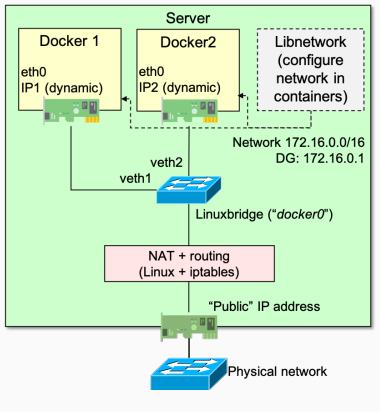
\includegraphics[scale=0.5]{images/docker private network.png}
    \caption{Docker network}
    \label{fig:dckrntwrk}
\end{figure}

\myparagraph{Union file system}
Containers must replicate the file system in order to have their replica. In this way they can guarantee isolation and portability. But how to do that? In fact file systems are quite large and they will require a huge download time and starting a process will become a slow operation. Docker offers a solution:

 The \textbf{Union File System} is a union of merged file systems with a single root. With this technique docker split two layers. a lower layer (read-only) and an upper layer (writable).
If a process wants to modify existing data, OS will copy data just for that process (Copy and Write technique). Simulation is used to hid the entire data and show it with the modifications requested. In this way only differences are stored and you don't need to copy all the bin and libs.

\begin{figure}[h!]
    \centering
    
\includegraphics[scale=1.5]{images/king.png}
    \caption{L'unico ed inimitabile Domenico, uno di noi}
    \label{fig:king}
\end{figure}
\clearpage
    \section{Cloud Networking}


\subsection{Data center networks}
    How to build a datacenter infrastructure? Let's have an introduction.
    
    \subsubsection{Cloud and networks}
        Cloud computing service, in order to offer a cloud service, has to be able to:
        \begin{itemize}
            \item virtualize hardware
            \item communicate with other structures (networking)
            \item to store information (storaging)
        \end{itemize}
        Now we want to focus on networking. Of course, working with lots and lots of data, if the bandwidth is limited, all the service will lose in efficiency. Moreover, more the data travel farther from the CPU data, more the latency will be a "bottle cone".

        In general there are at least three types of domain in networking:
        \begin{itemize}
            \item Peering domain where two networks exchange  have free relation of communication with each other
            \item Transitive domain where a provider network get payed  for transferring connectivity trough domains (The IXP)
            \item Customer domain where a customer network pay another network to get Internet access (The ISP)
        \end{itemize}
        
        Network are then classified in:
        \begin{itemize}
            \item Tier 1: reach every other network on the internet without paying or purchasing IP transit
            \item Tier 2: can be connected each other by means of an IP transit to reach some portion of the Internet (service providers)
            \item Tier 3: have to pay Tier 2 networks to go to on the Internet
        \end{itemize}
        \begin{figure}[h!]
            \centering
            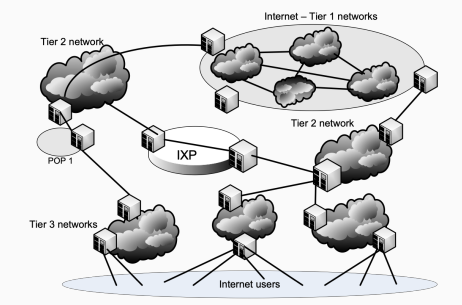
\includegraphics[scale=0.6]{images/network tiers.png}
            \caption{network tiers (nowadays an old model)}
            \label{fig:nettiers}
        \end{figure}
        
    \subsubsection{history}
        Over the time things changed and content-delivery network reshaped the definition of a network. At a certain point content providers had to deal with a growing demand of streaming services (because devices had become less expensive). That was a big problem because the network bandwidth was quite limited and content providers needed to guarantee the quality of their services (requesting more bandwidth). The main cause of this problem was the link connecting homes to the ISPs (called "last mile").
        
        Over years there has been a competition between national backbones (like Telecom Italia) and some big companies that created their own data centers and infrastructures.
        
        \FloatBarrier
        At the beginning, in fact, there where some national backbones operators that, thanks to some regional access providers and local access providers, brought Internet to costumers

        \begin{figure}[h!]
            \centering
            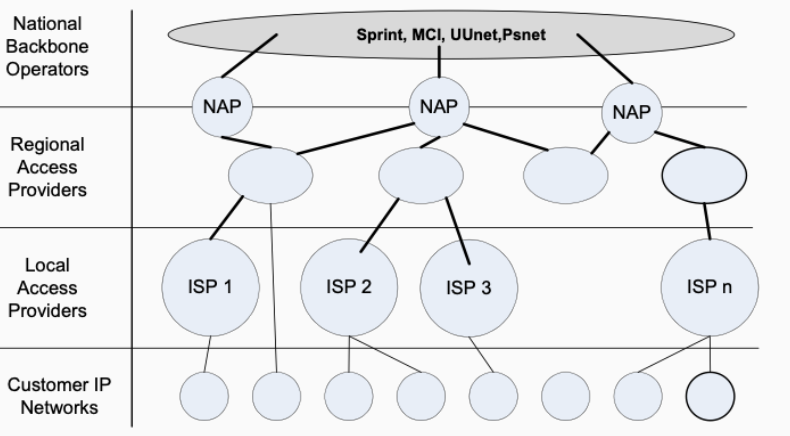
\includegraphics[scale=0.3]{images/providing structure 1.png}
            \caption{providing structure in 2007}
            \label{fig:nettiers}
        \end{figure}
        \FloatBarrier
        
        With the increased demand of services and bandwidth some hyper giants build their own structures and data centers everywhere and started providing their services.
        
        \FloatBarrier
        Nowadays the two entities works at the same time thanks to some Internet Exchange Points (IXP) that allows different ISP to exchange their Internet traffic each other.
        \begin{figure}[h!]
            \centering
            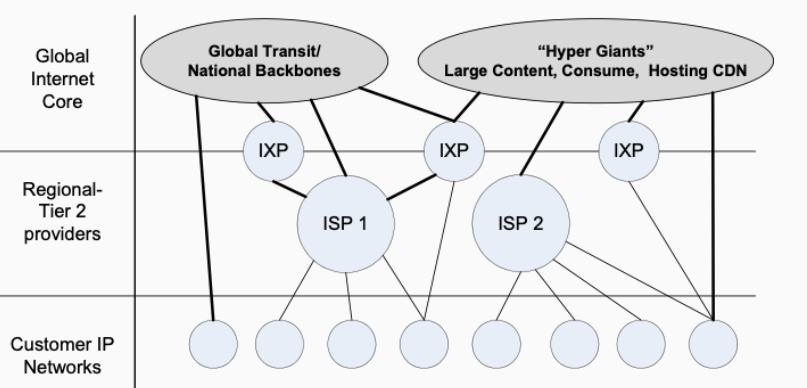
\includegraphics[scale=0.3]{images/providing structure 2.png}
            \caption{providing structure in 2009}
            \label{fig:nettiers}
        \end{figure}
        \FloatBarrier
        
        Google found another way of offering its service: it entered in some agreements with Telecom Italia to gets portion of Telecom Italia infrastructures to provide cloud services. In this way they didn't need to build new infrastructures spending more money.
        
        %Service provider is different form connectivity provider!
        
        
    \subsubsection{Characteristics}
        All modern data-centers shares some characteristics:
        
        Nowadays data center are structures with lots and lots of switches and routers (huge scale) that work with \textbf{high bandwidth} and with \textbf{very low round trip time}. From the point of view of the structure, they are quite homogeneous (they tries to have the same hardware [COTS]), with a regular topology and limited area occupations.
    
        However there are many aspects that can be changed:  the administrative domain, the routing, addressing and so on.
        % in some infrastructure there are paths that have the same costs that you can chose to use).
    
    
    \subsubsection{Requirements}
        In terms of requirements:
        \begin{itemize}
            \item Data centers work with lots of different connection flows. They must take care of both mice and elephant flows, it's need a low-latency user interaction.
            \item Data centers can work for a single and specific application (Google, Facebook, ...) or for some cloud service.
            \item Data centers works with two traffic directions:
            \begin{itemize}
                \item Outward, serving web pages to users
                \item Internal computation. Computation between data center is increasing more and more in relation with computation of user with data centers
            \end{itemize}
            \item Data centers often work with unpredictable workloads
        \end{itemize}
        
        
    \subsubsection{interconnection networks}
        A network is characterized by a common ensemble of elements that consists in:
        \begin{itemize}
            \item a set of nodes (processors, memory units, servers)
            \item links or communication channels
            \item a routing protocol used across nodes
            \item a flow control to menage congestions (usually in TCP level)
        \end{itemize}
        
        Switches are the components that receive data packs, identify the destination and uses routing tables to forward data packs until the destination. Thanks to them we can distinguish two network topologies:
        \begin{itemize}
            \item Static networks (direct connections between servers). Examples are: Bus, Hypercube, 2D-mesh and Torus topologies.
            \item Switched networks (switches are used to interconnect servers). Examples are crossbar and Omega switches
        \end{itemize}
        The topology will determine:
        \begin{itemize}
            \item the Network diameter
            \item the bisection width (if you cut the network at a certain point, is the minimum number of cuts to reach two halves)
        \end{itemize} 

        
    \subsubsection{Cloud interconnection networks}
        On top of servers there are some \textbf{aggregate switchers} that connect all servers. They can be optical or eletrical. Over them there is another layer of \textbf{core switches}.
        Ideally every server should be able to communicate with every other server with similar speed and latency.
        
        Yet Servers are largest amount of cost in a data center. So reducing it there will be a huge save of money.
        
        So the requirements for cloud interconnection are: Scalability, low cost, low-latency, high bandwidth and location transparent communication\footnote{Every server should be able to communicate with every other server with similar speed and latency}.
        
        
    \subsubsection{Conventional data center network}
        Every data center owner accord the design of it and the layers. In particular he can chose if working with layer 2 or layer 3.
        \begin{itemize}
            \item Playing with layer 2 allow working with fixed addressing and auto-configurations (much easier). However it has some limitations in the broadcast scale (ARP limitations)
            \item Playing with layer 3 guarantees more scalability through addressing and allow working with multipath routing (with equal costs). However it's more complex and do not guarantee migration without changing IP addresses
        \end{itemize}
        %We usually call POD (different from kubernetics) the layer 2.
        
        \FloatBarrier
        Data center looks as a giant switch that guarantee every connectivity (going from a server to another).
        Data center adopt the Clos topology that's base on  multiple stages. They are basically two butterfly networks that are inverted. It looks like a upside down fat tree.
        \begin{figure}[h!]
            \centering
            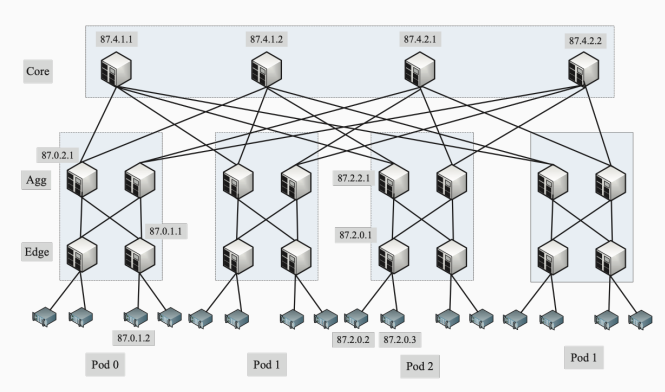
\includegraphics[scale=0.4]{images/clos topology.png}
            \caption{Clos topology}
            \label{fig:nettiers}
        \end{figure}
        \FloatBarrier
        
        Design principles:
        \begin{itemize}
            \item there are many of possible paths that cross exactly the same mount of links to go from one node to another
            \item the network can scale easily by changing some parameters
            \item multiple core switches
        \end{itemize}
        
        The main advantage of working with fat trees is that they are an optimal interconnection for large-scale clusters. In this cluster the servers are placed at the leafs, switches populate the root and the internal nodes of the tree. This is super regular and all switching elements of a fat-tree are identical.
        It's regular also in the number of elements: given the parameter $k$, you will have have $k$ pods; each pod has two layers; each layer has $\frac{k}{2}$ switches; each switch in the lower layer has connected to $k$ layers; every switch is connected to the aggregation layer. 
        
        Switches and pods are numbered and accessed by an IP address.
        
        There are some open issues to manage:
        \begin{itemize}
            \item There are different type of workloads with different requirements:
            \begin{itemize}
                \item Small flows (mice flows) requiring low-latency
                \item Large flows (elephant flows) requiring high-throughput
            \end{itemize}
            A datacenter needs a way of balancing them in order to provide to both of them a good service.
        
            \item Another issue is that TCP does not perform well in data center networks (we have to replace it with for example \textit{QUIC} or other networking protocols).
        \end{itemize}
        
        
        there are many equal costs path to go form one point to another. There are random allocated paths. The problem can be is that it doesn't care on resources occupation. May happens that if you have multiple elephant flow you may have collisions. If you have to elephant flows you have no problem. You can have collision also in the downward path. How do you menage flows within a data center network? There's research on this, quite advanced.
        
    \subsubsection{How to balance traffic flows}
        Assuming we want to go from the point S to the point D, there are many flows possible with equal cost path. Assuming that there's just one path down from each core switch:
        \begin{figure}[h!]
            \centering
            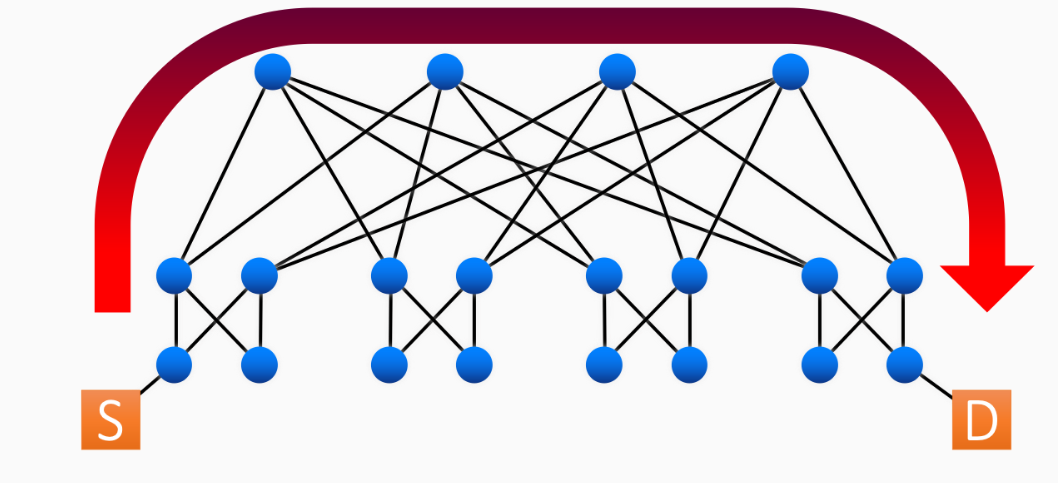
\includegraphics[scale=0.15]{images/trafficflow1.png}
        \end{figure}   
        
        The routing strategy to menage flows that is applied is \textbf{ECMP} (\textit{Equal-Cost Multi-Path}) that provides that paths are randomly allocated to flows (using hash of the flow).
        This routing strategy has the problem of not considering the limitation of available resources and can cause long lasting collision between elephant flows.
        
        To avoid this problem we can use Hedera, a scheduling technique that tries to detect elephant flows, computes non-conflicting paths and instructs switches to reroute traffic.
        
        There are many other possible solutions:
        \begin{itemize}
            \item Rerouting based on link utilization (but with the disadvantage of affecting mice flows)
            \item Rerouting based on switch queue occupancy, in particular removing elephant flows (that fill the most queues) and moving them away (but with the disadvantage of huge computation required)
            \item Spreading all packets uniformly (but with the disadvantage of more complicated TCP controls)
            \item Someone even proposed to change directly the TCP protocol
        \end{itemize}

    
    \subsection{Networking in virtualized environments}
        \FloatBarrier
        After creating multiple virtualized environments on a server (VMs, lightweight environments, containers), we need a sort of software bridge within the server that links their virtual network card to the virtual switch created by the OS.
        \begin{figure}[h!]
            \centering
            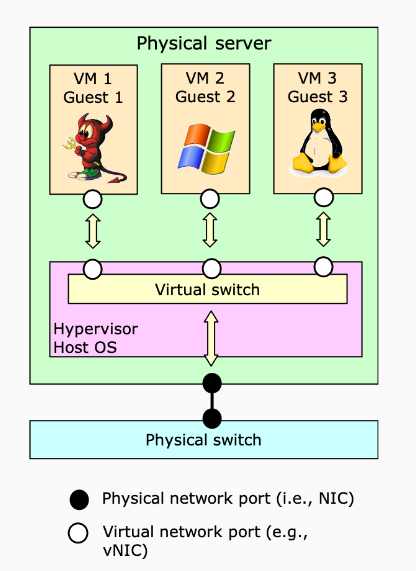
\includegraphics[scale=0.25]{images/virtualnet.png}
        \end{figure}
        \FloatBarrier
        
        From the point of networking, virtualization introduces additional complexity: in fact we need to deliver traffic from virtual to physical network (and vice versa) and between VMs/LXCs (within the same server).
        An additional requirement is to assign IP addresses to VMs/LXCs and provide advanced features such as load balancing, firewall ecc.
        
        In order to do this we need at first to provide Ethernet (L2) connectivity to VMs/containers and then to provide IP connectivity to them.

    
    \subsubsection{North/South and East/West communication on a single server}
        \FloatBarrier
        We can solve the problem presented above with at least three methods:
        \begin{itemize}
            \item Virtual (software) switch embedded in the OS
            \item In the NIC (using the physical network interface card and going back to the VM)
            \item In the external switch (getting out of the server, reaching the physical switch and the coming back)
        \end{itemize}   
        \begin{figure}[h!]
            \centering
            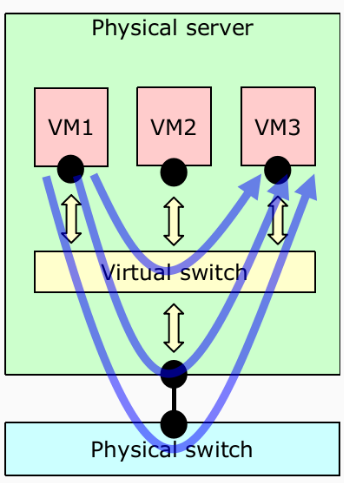
\includegraphics[scale=0.25]{images/virtserver.png}
        \end{figure}
        \FloatBarrier

        
        \myparagraph{Host-based switching}
            Historically the first solution ever used and the easiest one is \textbf{host-based switching} (or \textit{software bridge}). This solution works very well because the traffic is managed inside the server (high bandwidth) using some function given by the kernel without using the Internet layer (that has less capacity).
            One disadvantage is that it generates additional processing overhead and consumes CPU cycles. Another disadvantage is that it requires an additional component.
            Anyway this is the currently most common solution.
            
            Let's go deeper.
            
            The kernel is not a continuos process but it's triggered and reacts to events (event-based) that can be interrupts, system calls and whatever to interact.
            When a packet arrives a driver calls some functions of the kernel that menages packet. These function are called \textit{ETH Input} and they call \textit{IP Input} functions. These last function calls \textit{IP Forward} functions that understands where to sand packet by checking the routing table. 
            
            From a physical point of view, packets are moved by copying them from one VM in a space of memory reserved to the kernel and copied again in the second VM.
            
            A software bridge can be considered as an another function that is called to handle a packet on the layer 2. So a set of specific packets from virtual interfaces, instead of calling \textit{IP Input} functions, can go from \textit{ETH Input} functions to directly the Software bridge function at level 2.
            
            After that the bridge handles packets and calls the \textit{ETH Output} function which basically sands packets to a specific virtual interface of the machine.
            
            In addition, with software bridges you can apply policy directly in the virtual switch, intercepting the traffic before of other solutions.
            
            
        \myparagraph{Hairpin switching}
            The Hairpin switching use hardware that is already present (that has to be compatible).
    
            In particular packer are sanded to the physical switch and then received back in other VMs.
            
            It's slower then the previous one but don't use CPU cycles. Anyway This solution it's no longer used.
            

        \myparagraph{NIC switching}
            An intermediate solution is the NIC switching (intermediate also in terms of strengths and weaknesses). 
            
            In this solution we use some bridges called NICs in order to connect directly to the physical switch. These can be considered part of the network infrastructure because they are not controlled by the OS (and don't use the CPU capacity).
            
            In this way NICs avoid the problem about who controls edges switches.
            
            Another advantage is that, dedicating to NICs the job of transmitting packets, prevent DDoS attacks to affect these packets.
            
            In conclusion NICs gave the opportunity to researchers to  create smartNICs\footnote{A NIC with a processor and memory (like a GPU)}.
            

    \subsection{Software bridges in Linux}
        A software bridge provide intra-host connectivity to execution containers and handle IP addresses differently from the "official" IP model avoid the assignation of IP addresses to each network interface card (as opposed to the one IP address per NIC rule).
        
        \FloatBarrier
        A schema of basic bridging networking in Linux is the following:
        \begin{figure}[h!]
            \centering
            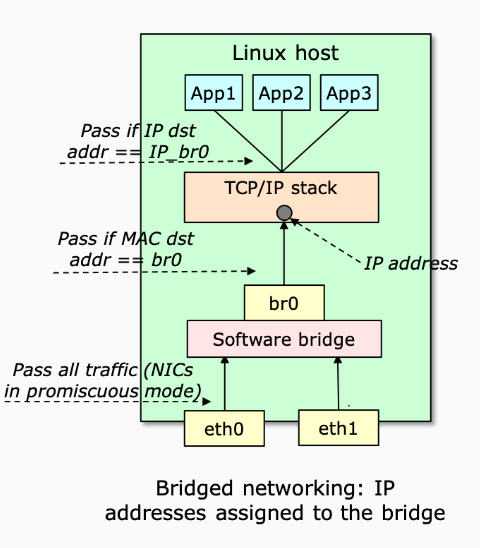
\includegraphics[scale=0.25]{images/bridgeschema.png}
        \end{figure}
        \FloatBarrier
        
        In order to avoid multiple IP addresses for each VM, the network interface card can be configured in a promiscuous mode. In this way every packet that is not intended for the machine MAC will be sand to the TCP/IP stack (crossing the internet interface transparently).
        
        Linux has three main types of software bridges:
        \begin{itemize}
            \item Linuxbridge
            \item Macvlan
            \item Open vSwitch
        \end{itemize}
    
    \myparagraph{Linuxbridge}
        Linuxbridge is the most common and simple one. It's a standard software provided by Linux that has everything that a physical switch needs; so it behaves like a traditional hardware switch (NICs has to be in promiscuous mode).
    
    \myparagraph{Macvlan}
    
        We define \textit{vlan} a broadcast domain (group) of ports used to partition lan in order to have a level 2 separation and isolation.
        
        Macvlan implements a VLAN-like behavior by using MAC addresses instead of tags. Macvlans look like a L2 interface with a personal and distinct MAC address (they can have a distinct IP address too).
        
        Macvlan support some operating modes:
        \begin{itemize}
            \item Private: makes a VLAN-like behavior; two macvlan belonging to different broadcast domains communicate thanks to routing.
            \item Virtual Ethernet Port Aggregator (VEPA) - Default mode: allows MAC A to talk with MAC B only if the traffic comes from the external world (so a switching element is required)
            \item Bridge: macvlan driver acts like a bridge; it's simple and fast
            \item Pass-through: it basically works by assigning directly cards to VMs (not much used)
        \end{itemize}
  
        
        \subsubsection{Open vSwitch}
        Open vSwitch is a software implementation of a virtual multilayer network switch that you can configure by using protocol used with real switches (so you can directly decide what to do with packets). It's much more complicated.
    
    
    \subsection{Single server: complex services}
        From a high level point of view, there are still some problem in attaching VMs to a virtual switch:
        \begin{itemize}
            \item what are the IP addresses provided to VMs? How to assign them?
            \item More network services may be required besides setting up bridge
            \item How to provide multi-tenancy? (multiple isolated environments that can communicate each other dedicated to multiple people in the same server or in different servers too). Tenants than can require additional networking services
            \item A NAT and a routing table is required too (connectivity is much complex than a single switch).
            \item How to manage TCP/IP stack?
        \end{itemize}

    \subsubsection{IP address assignment}
        The first problem to solve is how to assign IP addresses. There are different possible ways of doing it:
        
        \begin{itemize}
            \item The first option is \textbf{direct routing} that uses some IP addresses known by the physical network. This solution can be implemented in two ways:
            \FloatBarrier
            \begin{itemize}
                \item \textbf{Bridged mode}: VMs ask for IP addresses directly to the physical network. So VMs are directly attached to a vSwitch. In other words VMs rely on a upstream DHCP server to receive an IP address
                \item \textbf{Routed mode}: in this mode VMs ask for an IP to a vSwitch linked to a vDHCP server; so the router must know that to reach VMs it has to reach a vSwitch before
            \end{itemize}
            
            \begin{figure}[h!]
                \centering
                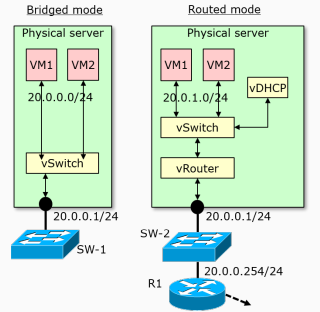
\includegraphics[scale=0.55]{images/IP ass.png}
            \end{figure}
            \FloatBarrier
            
            Pros of direct routing is that no NATting service is require because inbound and outbound connections are the same.
            
            Anyway it has many problems: how many IP addresses can be assigned? Than it will require the coordination of the network manager too. These cons made this solution not really the most used.
            
            Coordination with the network manager is required because we can't configure by ourselves router tables (that have information about directly attached network and other routers that can be used to reach networks not directly attached)
            
            \item The second option is \textbf{NATTed mode} that uses a vDHCP service to provide a private IP addresses to the VM (as it was a private network). vSwitch and vDHCP can be managed by the tenet.
            
            The connection to the Internet is than allowed by a NAT service. In fact there's a vNAT that changes private IPs (10.0.0.0) into Internet traffic (20.0.0.0).
            
            An advantage with this method is that no coordination with the network manager is required.
            
            A cons is that VMs are reached with different IPs (private or public) depending if the sender is inside or outside the private network.
            
            This model is used by Docker uses this model.
        \end{itemize}
        
        
    \subsubsection{Providing feature-rich network connectivity}

        To connect a VM to the physical infrastructure additional network services may be required (Router, NAT and DHCP for using private addresses). All these services are usually provided by by Linux itself or can be installed.
        
        In Docker there's some kind of DHCP service that works with the same concept but without using that exact protocol.
        
        
    \subsubsection{multi-tenancy}
        \FloatBarrier
        The solution for supporting multiple tenents on a physical server is to use as many vSwitch and vRouters as many tenets I need.
        
        This approach is preferred to vLANs because it is completely software based and it's easier to configure and manage rather than vLANs.
        \begin{figure}[h!]
            \centering
            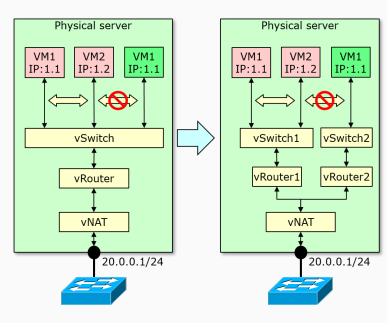
\includegraphics[scale=0.55]{images/multi tenancy.png}
        \end{figure}
        \FloatBarrier
        
        
        
    \subsubsection{Tenant-defined network services}
        \FloatBarrier
        A single tenet may want pretty complex services like having multiple machines but exposing just one to the vSwitch through a L7 firewall (in order to defend the VM and to filter possible queries); So the tenant can create more complex service on its own. It can use Linux provided functionality or functionality provided by some installations.
        \begin{figure}[h!]
            \centering
            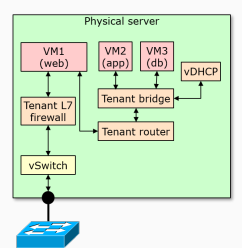
\includegraphics[scale=0.4]{images/tenant services.png}
        \end{figure}
        \FloatBarrier
        
        
    \subsubsection{Co-existence of virtual services and host applications}
        \FloatBarrier
        Within the server we have a TCP/IP stack (used with some applications that run on the server) that need to coexist with VMs.
        \begin{figure}[h!]
            \centering
            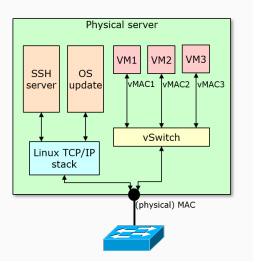
\includegraphics[scale=0.55]{images/TCP IP stack.png}
        \end{figure}
        \FloatBarrier
        
        In particular in order to distinguish inbound traffic toward VMs the physical interface on the server use hardware filtering: a packet that arrives with a MAC address not recognized will be dropped.
        
        In a bridged mode, MAC addresses will be different from the physical one, so we need to configure the physical card to be in promiscuous mode. This is not needed if using a vRouter NAT.
        Than inbound traffic is recognized by using different MAC addresses (otherwise we can use ports or use some intelligent software).
        
    
    \subsubsection{vNIC}
        Supposing that a VM want to send a packet, how to understand if it's for the Internet or for another VM?
    
        A \textbf{vNIC} is a device driver that connects VMs with the Linux IP stack and with the vSwitch (it can be implemented simply as a virtual ethernet interface).
        
        It's a network interface that is attached in the namespace where VMs are and links the root namespace (by facts it runs in the Linux kernel). 
        
        When the vNIC receives a packet it detects the destination of it. If it's the Internet, it sands it to the Linux IP forwarding module (technically to the default gateway). After that the kernel will manage it by looking to routing tables and using ARP protocol.
        
        \myparagraph{Practical example}
            Let's assume that the VM1 wants to sand a packet to the Internet. The packet that exits the VM has a source address 10.0.0.1 (MAC of the VM) and a destination address 8.8.8.8 (that's the MAC of the vNIC, learnt by a broadcast request) and it has to go via 10.0.0.254. This packet gets to the vSwitch that does a filtering forwarding. The packet is than sand to the vNIC that look to the destination: if it's not for the vNIC it will be sanded to the forwarding module of the kernel that will use a routing table and the IP address as a gateway.
        
        
    \subsection{DC-wide services}
    
        We want now to connect VMs across different physical servers. Thinking wide, when moving from a single server to a datacenter, the problems to solve are the same of VMs but with a different scale (datacenters can include thousand of servers): IP address assignments, supporting multiple tenants and so on.
        
        \FloatBarrier
        Let's distinguish two point of view:
        \begin{itemize}
            \item The tenet wants to deploy its virtual service ignoring the physical infrastructure (number of servers and connection between them); in fact VMs can be on different servers;
            \item The Cloud manager has to build the infrastructure that the Tenet uses.;
        \end{itemize}
        \begin{figure}[h!]
            \centering
            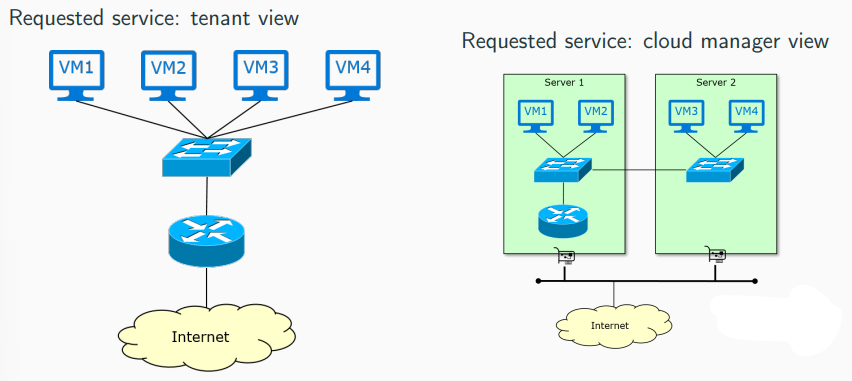
\includegraphics[scale=0.55]{images/point of views.png}
        \end{figure}
        \FloatBarrier

    \subsubsection{Providing L2 connectivity to tenant services across DC}
    
        Let's assume that a costumer wants to have a L2 network among all its services (VMs). In order to allow that, the Cloud manager needs to create a tunnel between switches of servers.
        
        
        
        L2 connectivity to services of tenents across different machines or L3 connectivity. This is a decision of the customer, depending on what he wants. We want all VMs connected as i would have a L2 connection. We need to create a tunnel between switches of servers.
        From the point of view of the cloud manager we have multiple servers with different VMs over them.
        In a physical environment i would have some machine and a switch. In virtual world is different. 
            
        \FloatBarrier
        Let's assume that a tenant has VM1, VM2, VM3 and VM4 and that he wants them to be connected as they was in a bridged network (it doesn't know they are in different servers).
        \begin{figure}[h!]
            \centering
            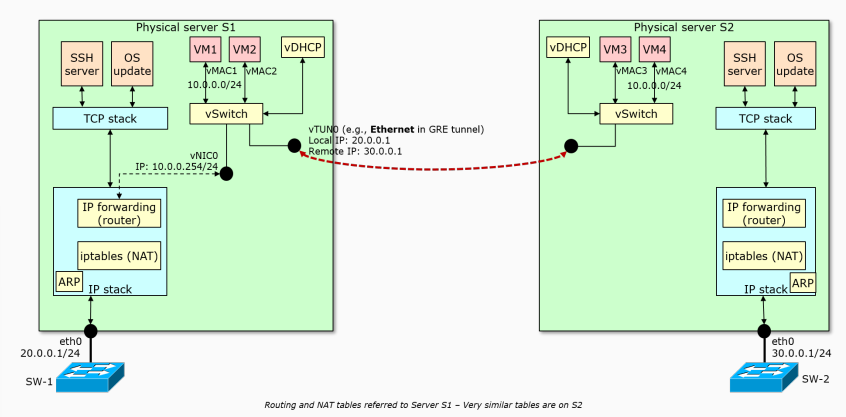
\includegraphics[scale=0.5]{images/example of tunneling.png}
        \end{figure}
        \FloatBarrier
        
        In real world different machines could be connected by using two switches connected with an ethernet cable.
        
        The same happens in virtualized world: the Cloud manager creates a tunnel from a \textbf{vTUN0} interface (that has the same characteristics of an internet interface). The VTUN0 uses the \textbf{GRE protocol}; in particular it encapsulates frames or packets, add some small in-layers and another IP header with the localIP (source) and the remoteIP (destination).
        As result, we connected two machines with a L2 connection.
        
        With this connection the vNIC in the second server is no longer required: packets sanded from VM3 and VM4 can use pass trough the vTUN0 and use the vNIC0 of the first server.
        
        
    \subsubsection{Providing L3 connectivity to tenant services across DC}
        If a customer asks for a L3 connectivity without caring of the L2 one (neither about IP addresses), there are two possible working modes:
        \begin{itemize}
            \item tunneling
            \item direct routing
        \end{itemize}
        
        \FloatBarrier
        In \textbf{tunneling} a tunnel directly attached to the IP forwarding router is used. This tunnel will use the \textbf{IP in GRE} protocol; so in the encapsulation phase the IP packet will be put in another IP packet (so the tunnel needs to have a dedicated IP address).
        The first IP header will be than removed on the server 2.
        \begin{figure}[h!]
            \centering
            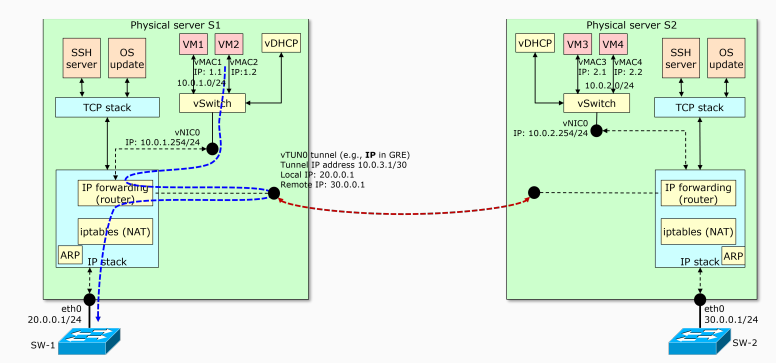
\includegraphics[scale=0.5]{images/tunneling.png}
        \end{figure}
        \FloatBarrier
        
        A possible problem is that when doing encapsulation the packet size is increased (because of the addition of another header). This could be a problem if the packet have already reach the maximum size. The solution is fragmentation which however adds some overhead.
        
        \FloatBarrier
        Otherwise, if fragmentation is not acceptable, \textbf{direct routing} is the last solution. The packet will be sand outside of the S1 and trough a router will be received by the second switch that will sand to the S2.
        \begin{figure}[h!]
            \centering
            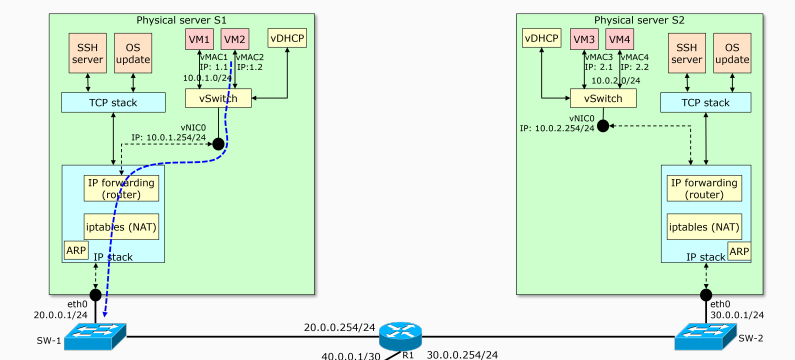
\includegraphics[scale=0.5]{images/direct routing.png}
        \end{figure}
        \FloatBarrier
        
        Summarizing:
        \begin{itemize}
            \item Overlay (tunneling)
            \begin{itemize}
                \item no interaction with the infrastructure is required
                \item adds some overhead (logical channels over physical ones)
            \end{itemize}
            \item Direct routing
            \begin{itemize}
                \item requires the collaboration of the infrastructure provider
                \item 
            \end{itemize}
        \end{itemize}
    \section{Cloud Storage}


\subsection{Storage models}
    In cloud computing a massive amount of data needs to be handled. If years ago the most important service was the performance of cloud, nowadays it' reliability: data has to be stored and providers have to be able to make sure to not lose them.
    In order to provide reliability, different copies of the same data will be stored. The disadvantage is that maintaining consistency among multiple copies of data will require more software complexity.
    
    We define \textbf{storage model} the layout of a data structure in a physical storage.
    
    We define \textbf{data model} the set of logical aspects related to how to store data in a given space.
    
    Storage models must guarantee two features:
    \begin{itemize}
        \item Storage models must be \textbf{read/write coherent}: the result of a read operation of memory should be the same as the most recent write operation; in other words every operation of read operation needs to ensure that the previous write operation has been already completed.
        \item Storage models must respect the \textbf{before-or-after atomicity}: the result of an operation, from the point of view of the invoker, must be the same as if the actions occurred either completely before or completely after.
    \end{itemize}

    
\subsection{Block storage}
    Data are managed by means of blocks within sectors and tracks (this is very useful mostly for databases by DBMS).
    
    OpenStack Cinder is a Block Storage service for OpenStack. It's designed to present storage resources to end users, in particular it allows to interact with different row and not formatted hardware. 
    
    \begin{figure}[h!]
        \centering
        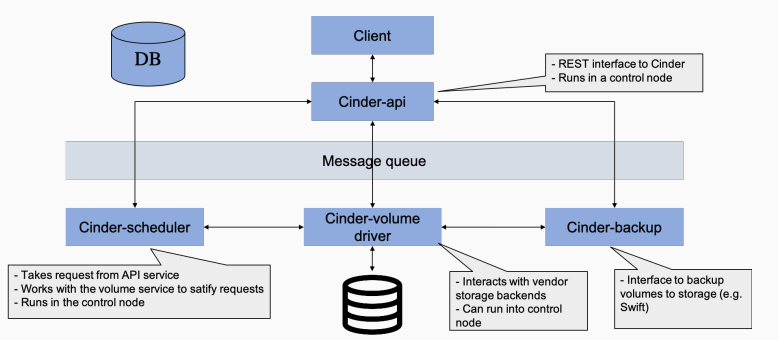
\includegraphics[scale=0.5]{images/Cinder architecture.png}
    \end{figure}
    
    The Cinder architecture is composed by:
    \begin{itemize}
        \item a volume driver that interacts with the vendor
        \item a scheduler that takes request from the API interface (like modifying a volume and snapshots).
        \item a backup that is an interface for backupping volumes.
    \end{itemize}


\subsection{Distributed file systems}
First of all, let's introduce some terms:
\begin{itemize}
    \item A \textbf{file} is a linear array of cells stored on a persistent storage device. From the point of view of applications it's viewed as a collection of logical record and is stored on a physical device as a set of physical records of size determined by the physical media.
    \item A \textbf{file pointer} is a cell used as a starting point for a read or write operation of a file.
\end{itemize}
Files could be organised as:
\begin{itemize}
    \item \textbf{Logical}: the organization reflects the data model. This is often the prospective the applications.
    \item \textbf{Physical}: the organization reflects the storage model and describes the manner the file is stored on a given storage media.
\end{itemize}

So a \textbf{file system} is a collection of directories (logical partition of the disk) and each one provides information about the organization of a set of files.
File system can be \textit{traditional} (like the Unix File System) or \textit{distributed} (like the Network File System ...).


\subsubsection{Unix File System}
The \textbf{Unix File System} (UFS) is based on three main points:
\begin{itemize}
    \item It's designed a \textit{layered} mode; this provides flexibility because:
    \begin{itemize}
        \item It allows UFS to separate the concerns for the physical structure (hardware) from the logical one (applications).
        \item \textit{inode} layer allows UFS to treat uniformly local and remote file access.
    \end{itemize}
    \item Its \textit{hierarchical} design supports scalability reflected by the file naming convention (like nested directory)
    \item \textit{Metadata} supports a systematic design philosophy of the file system and device-independence
    \begin{itemize}
        \item Metadata includes information like file owner, access rights, creation time etc. (information useful for managing files)
        \item \textit{inodes} contains information about individual files and directories
    \end{itemize}   
\end{itemize}   

\myparagraph{USF layering}
Lower layers are dedicated to the physical organization:
\begin{itemize}
    \item A \textit{Block layer} locates individual blocks on the physical device;
    \item A \textit{File layer} reflects organization of blocks into files;
    \item A \textit{Inode} layer provides metadata for the objects;
\end{itemize}

Upper layers are dedicated to the logical organization.

Than there's the File name layer (I/O layer) that mediates between machine and user oriented view of the FS. In particular it provides an API to allow communication between them.

\begin{figure}[h!]
    \centering
    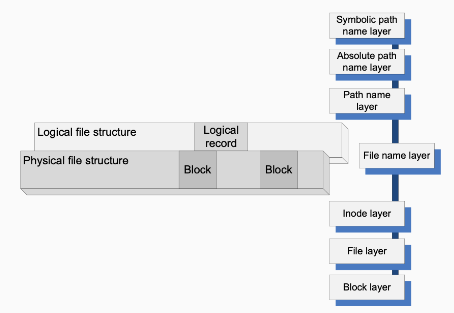
\includegraphics[scale=0.35]{images/UFSlayering.png}
    \caption{UFS layering}
    \label{fig:usfl}
\end{figure}


\subsubsection{Network File System}
The \textbf{network file system} (NFS) has been the first which was distributed. It has been created to have a sort of integration with the UFS.

Its design objectives are:
\begin{itemize}
    \item Provide the same semantics as a local UFS to ensure compatibility.
    \item Facilitate the integration into existing UFS.
    \item Support clients running on different operating system.
    \item Accept a modest performance degradation due to remote access.
\end{itemize}

NFS is based on the Client-Server paradigm: a Client runs on the local host while the server is at the site of the remote file system. Client and Server interact by means of Remote Procedure Calls (RPC).

In the NFS remote files are uniquely identified by a file handler (instead of a file descriptor).
\begin{figure}[h!]
    \centering
    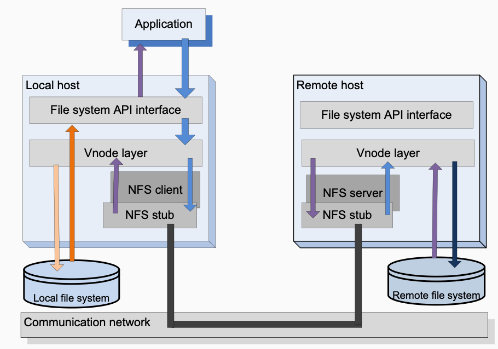
\includegraphics[scale=0.35]{images/NFS.png}
\end{figure}

On the local host and on the remote host there's a \textbf{vNODE layer} (corresponding of inode) that implements file operations in a uniform manner, regardless of whether the file is local or remote.

The mechanism of the client-server interaction in steps is:
\begin{itemize}
    \item An application request for a file;
    \item the vNODE layer of the remote host tries to understand if the file is local to the remote host or not;
    \item if it's not local, it will requests for it from the local host;
    \item the vNODE layer of the local host will receive the request for the file;
    \item if the file is present, the vNODE layer will sand it to the remote host;
    \item the vNODE of the remote host will direct the file to the remote file system.
\end{itemize}


\subsubsection{Design choices for distributed file system}
Distributed file systems have common features:
\begin{itemize}
    \item Common policy: conventionally when a file is close, the server should have the newest version on persistent storage;
    \item Policy to write a block:
    \begin{itemize}
        \item in \textit{write-backs} policy a block is first written to cache while the writing on the disk is delayed for a time (tens of seconds). This policy speeds-up the writing operation but it can cause data loss if the system fails;
        \item in \textit{write-through} policy a block is written to the disk as soon as it's available on the cache. This policy increase reliability but requires more time to complete the writing operation;
    \end{itemize}
    \item Concurrency:
    \begin{itemize}
        \item in \textit{sequential write-sharing} a file cannot be opened simultaneously for reading and writing operations by several clients (preferable). This policy is allowed by some unique access algorithms that can locks files;
        \item in \textit{Concurrent write-sharing} a file can be opened and modified by multiple clients (often not acceptable);
    \end{itemize}
    \item Parallel I/O executions: if allowed, it implies the execution of multiple input/output operations. To allow the parallel execution, the concurrency need to be handled in some way.
\end{itemize}


\subsection{General Parallel File System}
The \textbf{General Parallel File System} (GPFS) is the first file system invented. It's structured in some servers connected with LANS.

\begin{figure}[h!]
    \centering
    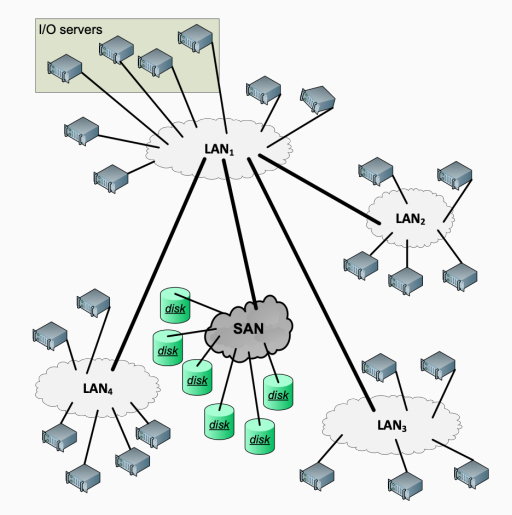
\includegraphics[scale=0.35]{images/GPFS.png}
    \caption{GPFS}
    \label{fig:gpfs}
\end{figure}

One important feature that GPFS introduced is a method of handling potential error: GPFS records all metadata updates in a log file that can be used to retrieve back information if errors on the file system occur.

One problem of the GPFS system is data striping that provides the segmentation of data. This policy improves performances (because it allow concurrent access) but since data are segmented and stored in different places, when the disk fails, a large number of files are affected.


\subsubsection{Google File System}
The \textbf{Google File System} (GFS) was developed in the late 90s.
Its design has the following features:
\begin{itemize}
    \item Scalability and reliability are critical. These aspects are because GFS uses thousands of storage systems to provides petabytes of storage to a large user community;
    \item The majority of file sizes range from few GB to hundreds of TB;
    \item Most common operations in the GFS are reading and appending something to existing files;
    \item Sequential read operation;
    \item Since file sizes are quite large, files are segmented in large chunks (that work with the TCP connection protocol).
    
    Chunks are fixed-size segments of 64 MB. They are quite large because:
    \begin{itemize}
        \item they work well with large files;
        \item they reduce the total metadata (less files means less metadata);
        \item multiple likelihood operations will be directed to the same chunk (so you can work inside the same chunk with less overhead; this means working with the same server);
    \end{itemize}
    Chunks are stored on Linux File System and are replicated on multiple sites.
    
    At the time of file creation each chunk is assigned a unique chunk handle. They are put in chunk servers (every chunk server is assigned to a set of chunks and uses a communication network to work with the master);
    \item GFS builds cluster around high-bandwidth (and it separates the control flow from data one); 
    \item Eliminates caching at the client site (leaving it only on the server side);
    \item Have a master that controls the entire cluster (it will maintain state information about all the system components) in order to "enter" the cluster", we have to communicate with it. The master node is the mechanism that allows consistency;
    \item GFS introduced checkpointing, recovering and a garbage collection system.
\end{itemize}

\begin{figure}[h!]
    \centering
    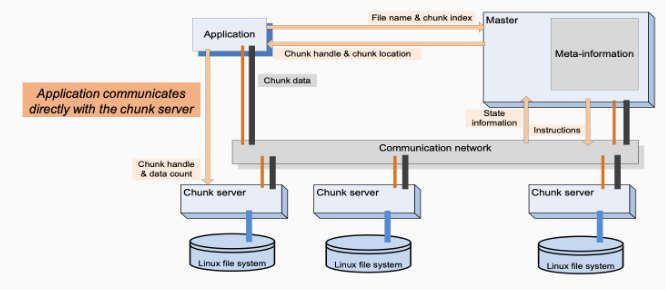
\includegraphics[scale=0.35]{images/GFS arch.png}
\end{figure}

Let's see how a write request is performed:
\begin{itemize}
    \item The client contacts the master which assigns a lease to one of the chunk servers; 
    \item The master replies with the ID of a primary and secondary chunk servers (that hold replicas of the chunk);
    \item The client sends data to all chunk servers that hold replicas (using the chunk handlers);
    \item Once it got an ack from all chunk server that hold replicas, the client send a write request to primary chunk server; 
    \item Primary chunk server sends the write request to all secondaries;
    \item Each secondary applies mutations in the order of the sequence number and sends ack back to primary;
    \item After receiving ack from all secondaries, primary sands an ack to the client.
\end{itemize}


\subsection{Locks and consensus}
Operating systems use lock managers to organise and serialise access to resources. In particular locks enable controlled access to shared storage and ensure atomicity of read and write operations (to avoid any collision).

Locks are allowed by the presence of a leader that is referred for getting information. It's elected through consensus. Election are implemented by a consensus protocol that accords everybody about a master.

To lock some resources we can use a distributed approach or a locking service (library to make process talk to each other asking for accesses).

The locks are discriminated for their effect:
\begin{itemize}
    \item \textbf{Advisory locks} are based on the assumption that all processes respects some rules (all file can have the access of the file);
    \item \textbf{Mandatory locks} block access to the locked objects to all processes that do not hold the locks;
\end{itemize}
and for the time:
\begin{itemize}
    \item \textbf{Fine-grained locks} can be held for only a very short time;
    \item \textbf{Coarse-grained locks} held the block for a longer time;
\end{itemize}


\subsubsection{Chubby}
Chubby is a very reliable and distributed lock service developed by Google for coarse-grained synchronization of distributed systems.
It's developed for a large number of machines connected by high-speed network and provides an interface much like a distributed file system.
It's an \textbf{advisory lock} and uses PAXOS\footnote{It's a family of protocols for solving consensus problems in a network} to ensure liveness.

The design of chubby it's not complicated and it consist of two main component that communicate via RPC (a replica server and a library).

Chubby cell consists of a small set of servers (typically 5) known as replicas that use PAXOS to elect a master and replicate logs. Read and write requests are satisfied by the master alone.
\begin{figure}[h!]
    \centering
    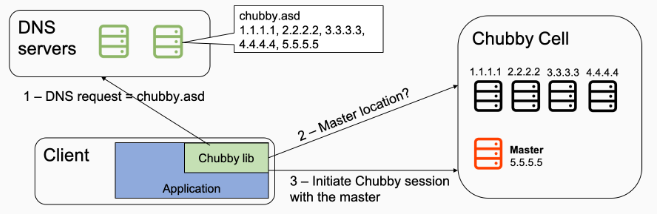
\includegraphics[scale=0.35]{images/chubbydesign.png}
\end{figure}

Chubby exports a file system interface, simpler than Unix, to provide some information. This file system interface is a tree of files and directories (with name components separated by /); each directory contains a list of child files and other sub-directories.
\begin{table}[h!]
    \centering
    \begin{tabular}{c c c}
          ls / & asd / & dunno/nothingJS\\
          is a prefix common & name of the & is the named chubby cell\\
          to all chubbys (lock service) & chubby cell 
    \end{tabular}
\end{table}

Chubby works with \textbf{nodes} that represent a file or directory. Each file can be either permanent or ephemeral and have some metadata and handlers associated to. In Chubby you can ask to open/close a node, to read/write contents and to  acquire/delete nodes.


\subsection{Distributed databases}
The \textbf{Google big table} (GBT) is a distributed storage system for managing structured data. 

Its design features are:
\begin{itemize}
    \item designed to scale to a very large size;
    \item not a relational database;
    \item designed as a key/value sorted and multi-dimensional map;
    \item flexible
    \item high performance solution
\end{itemize}

\begin{figure}[h!]
    \centering
    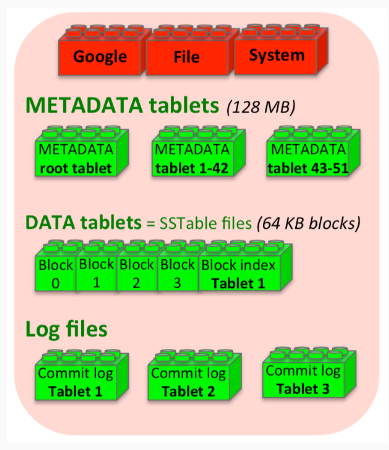
\includegraphics[scale=0.35]{images/GBTstruct.png}
\end{figure}

Being a sorted map, it has a set of columns associated with certain keys and a set of rows associated to entries (in form of strings of x bytes). Each cell is than a non interpreted array of bytes.

There's than a final dimension that's the timestamp with whom every information is recorded.

Rows are divided in groups of rows, called tablets.

The major components of GBT are:
\begin{itemize}
    \item One \textbf{Master} server that:
    \begin{itemize}
        \item assigns tablets to tablet servers;
        \item detects the addition and expiration of tablet server;
        \item balances tablet server load;
        \item does the Garbage collecting of files in GFS;
        \item handles schema changes.
        \item 
    \end{itemize}
    \item Many \textbf{Tablet} servers, each one:
    \begin{itemize}
        \item manages a set of tablets;
        \item handles read and write request to the tablets;
        \item splits tablets that have grown too large.
    \end{itemize}
    \item The \textbf{Client} that does not rely on the master (for tablet location and information) but instead communicates directly with tablet servers for reads and writes.
\end{itemize}

Each tablet is than assigned to one tablet server at time by the server (with a tablet load request to the server).
The tracking is realized by Chubby. So the Bigtable service works only if Chubby is available, otherwise it will be unavailable too.

When a tablet server starts, it creates and acquires an exclusive lock on a uniquely-named file in a specific Chubby directory.

Tablet server stops serving its tablets if it loses its exclusive Chubby lock. Master is responsible for detecting when a tablet server is no longer serving its tablets. To ensure that a Bigtable cluster is not vulnerable to networking issues if the master's Chubby session expires it will kills itself.

%QUESTA PARTE LA FINISCO DOMANI

\end{document}
